%% ============================================================
%%  NeuroMotion – EEG-Based Robotic Assistance System
%%  Alamein International University | BSc. CSE Graduation Project
%% ============================================================

\documentclass[12pt, a4paper, oneside]{report}

%% ── Packages ─────────────────────────────────────────────────
\usepackage[top=2.54cm, bottom=2.54cm, left=3.17cm, right=3.17cm]{geometry}
\usepackage{graphicx}
\usepackage{float}
\usepackage[section]{placeins}
\usepackage{setspace}
\usepackage{titlesec}
\usepackage{tocloft}
\usepackage{hyperref}
\usepackage[T1]{fontenc}
\usepackage[utf8]{inputenc}
\usepackage{lmodern}
\usepackage{parskip}
\usepackage{booktabs}
\usepackage{array}
\usepackage{microtype}
\usepackage{emptypage}
\usepackage{fancyhdr}
\usepackage{amsmath}
\usepackage{tikz}
\usetikzlibrary{arrows.meta,positioning,backgrounds,shapes.geometric}
\usepackage{xcolor}
\graphicspath{{./}}

%% ── Fonts & Spacing ──────────────────────────────────────────
\setstretch{1.5}
\setlength{\parindent}{0pt}
\setlength{\parskip}{6pt}

%% ── Hyperref setup ───────────────────────────────────────────
\hypersetup{
    colorlinks  = true,
    linkcolor   = black,
    citecolor   = black,
    urlcolor    = black,
    pdftitle    = {NeuroMotion: EEG-Based Robotic Assistance System},
    pdfauthor   = {AIU CSE 2026},
}

%% ── Chapter / Section title formatting ───────────────────────
\titleformat{\chapter}[block]
  {\normalfont\Large\bfseries\centering}
  {CHAPTER \thechapter:}{0.5em}{}
\titlespacing*{\chapter}{0pt}{0pt}{20pt}

%% ── ToC formatting ───────────────────────────────────────────
\renewcommand{\cftchapfont}{\bfseries}
\renewcommand{\cftsecfont}{}
\renewcommand{\cftchappagefont}{\bfseries}
\setlength{\cftbeforechapskip}{4pt}

%% ── Page style ───────────────────────────────────────────────
\setlength{\headheight}{14pt}          % suppress fancyhdr headheight warning
\pagestyle{fancy}
\fancyhf{}
\fancyhead[R]{\small\textit{NeuroMotion: EEG-Based Robotic Assistance System}}
\fancyfoot[C]{\thepage}
\renewcommand{\headrulewidth}{0.4pt}

%% ============================================================
\begin{document}

\pagenumbering{roman}

% ─────────────────────────────────────────────────────────────
%  COVER PAGE
% ─────────────────────────────────────────────────────────────
\begin{titlepage}
\thispagestyle{empty}
\centering

%% Place aiu_logo.png in the same directory as this file.

\includegraphics[width=5cm]{aiu_logo}\\[0.4cm]

{\Large\bfseries Alamein International University\\[0.15cm]
Faculty of Computer Science \& Engineering}\\[1.0cm]

{\LARGE\bfseries NEUROMOTION}\\[0.3cm]
{\large\bfseries EEG-Based Robotic Assistance System}\\[1.0cm]

{\normalsize\itshape
A project submitted in partial fulfillment of the\\
requirements for the BSc. degree}\\[0.9cm]

{\normalsize\bfseries By}\\[0.3cm]
{\normalsize
Mostafa Ibrahem Hasona \hfill (20100257)\\[0.2cm]
Youssef Ali Elsayed Ahmed \hfill (20100251)\\[0.2cm]
Youssef Mohammed Magdy Elbanna \hfill (21100841)\\[0.2cm]
Muhammad Sherif Muhammad Awad \hfill (22100638)\\[0.9cm]
}

{\normalsize\bfseries Supervised by}\\[0.25cm]
{\normalsize Dr. Ahmed Shalaby}\\[0.9cm]

{\normalsize\bfseries 2025 -- 2026}

\end{titlepage}

% ─────────────────────────────────────────────────────────────
%  ACKNOWLEDGEMENT
% ─────────────────────────────────────────────────────────────
\clearpage
\chapter*{ACKNOWLEDGEMENT}
\addcontentsline{toc}{chapter}{ACKNOWLEDGEMENT}

We would like to express our sincere gratitude to \textbf{Alamein International University (AIU)} for providing the academic environment and resources that made this graduation project possible.

We are deeply thankful to our supervisor, \textbf{Dr. Ahmed Shalaby}, for his continuous guidance, technical insight, and encouragement throughout both semesters of this project. His expertise in artificial intelligence and embedded systems was instrumental in shaping both the direction and the quality of our work. His door was always open, and his feedback always constructive.

We extend our appreciation to the research team at \textbf{Benha University}, led by \textbf{Eng. Heba El Shahat}, for generously sharing their raw EEG motor imagery recordings, which provided the experimental data foundation for our preprocessing pipeline development and system validation.

Finally, we thank the \textbf{Faculty of Computer Science \& Engineering} for the solid academic foundation that equipped us to undertake a project at the intersection of neuroscience, machine learning, and robotics --- and our \textbf{families}, whose unwavering support carried us through every late night and difficult milestone.

% ─────────────────────────────────────────────────────────────
%  UNDERTAKING
% ─────────────────────────────────────────────────────────────
\clearpage
\chapter*{UNDERTAKING}
\addcontentsline{toc}{chapter}{UNDERTAKING}

This is to declare that the project entitled \textbf{``NeuroMotion: EEG-Based Robotic Assistance System''} is an original work done by the undersigned, in partial fulfillment of the requirements for the BSc. degree at the Faculty of Computer Science \& Engineering (CSE), Alamein International University (AIU).

All analysis, design, system development, and implementation have been accomplished by the undersigned. This project has not been submitted to any other college or university.

\vspace{2cm}

\noindent
\textbf{Signed,}\\[1cm]
Mostafa Ibrahem Hasona\\[0.7cm]
Youssef Ali Elsayed Ahmed\\[0.7cm]
Youssef Mohammed Magdy Elbanna\\[0.7cm]
Muhammad Sherif Muhammad Awad

% ─────────────────────────────────────────────────────────────
%  ABSTRACT
% ─────────────────────────────────────────────────────────────
\clearpage
\chapter*{ABSTRACT}
\addcontentsline{toc}{chapter}{ABSTRACT}

% [HARDWARE-AGNOSTIC PARAGRAPH — describes the intended system design.
%  Revise or confirm wording before final submission]:
Millions of individuals worldwide suffer from motor disabilities that prevent them from
operating conventional assistive devices. NeuroMotion is a non-invasive Brain-Computer
Interface (BCI) system designed to enable real-time mental control of a humanoid robot
(HBE Robonova AI3) through EEG-based motor imagery classification. The system is
architected around a 14-channel EEG acquisition front-end, a signal preprocessing pipeline,
a machine learning classification layer, and a serial command interface to the target robot
platform.

The signal processing pipeline comprises bandpass filtering at 8--30\,Hz, zero-mean
normalisation, and temporal segmentation into stimulus-locked epochs. Feature extraction is
performed using Common Spatial Patterns (CSP), and classification employs a hierarchical
dual-SVM architecture to predict four directional mental commands: Forward, Backward,
Left, and Right.

A hierarchical ``divide-and-conquer'' classification approach was developed to overcome the
multi-class accuracy degradation caused by spatial overlap in EEG signals: \textbf{Model~A}
specialises in horizontal commands (Left vs.\ Right) and \textbf{Model~B} specialises in
vertical commands (Forward vs.\ Backward). A confidence gating mechanism rejects
predictions below a 60\% threshold to ensure operational safety.

The full pipeline was implemented in Python and validated through simulation using raw EEG
motor imagery data acquired and shared by a research team at Benha University, to which our
own preprocessing pipeline was applied. The backend communicates predicted commands to
the Robonova via Serial/UART, targeting a decision latency under 1.5 seconds. The GUI
(\textit{NeuroMotion::LINK}) provides real-time EEG visualisation, neural telemetry, and
manual override. AES Fernet encryption and API tokenisation secure all telemetry data.
Benchmarking against LDA, Random Forest, XGBoost, and KNN established SVM with RBF
kernel as the optimal classifier. Cross-user validation confirmed that user-specific calibration
is required for reliable performance.

% ─────────────────────────────────────────────────────────────
%  TABLE OF CONTENTS
% ─────────────────────────────────────────────────────────────
\clearpage
\renewcommand{\contentsname}{TABLE OF CONTENTS}
\tableofcontents

% ─────────────────────────────────────────────────────────────
%  LIST OF TABLES
% ─────────────────────────────────────────────────────────────
\clearpage
\renewcommand{\listtablename}{LIST OF TABLES}
\listoftables

% ─────────────────────────────────────────────────────────────
%  LIST OF FIGURES
% ─────────────────────────────────────────────────────────────
\clearpage
\renewcommand{\listfigurename}{LIST OF FIGURES}
\listoffigures

\clearpage
\pagenumbering{arabic}

% ─────────────────────────────────────────────────────────────
%  CHAPTER 1 — Introduction & Background
% ─────────────────────────────────────────────────────────────
\chapter{Introduction \& Background}

\section{General Topic and Importance}

Assistive technology has long played a critical role in improving the quality of life for
individuals with motor disabilities. Traditional interfaces --- joysticks, keyboards, and voice
control --- remain inaccessible to people with severe physical or speech impairments.
Brain-Computer Interfaces (BCIs) represent a paradigm shift: they allow direct communication
between the human brain and external devices without relying on muscular pathways.

NeuroMotion is a graduation project developed at Alamein International University that
addresses this gap by designing and implementing a real-time, non-invasive EEG-based system
for humanoid robot control. The system leverages established signal processing techniques,
machine learning, and an intuitive GUI to deliver a practical, accessible solution for users with
mobility impairments. The complete pipeline --- from raw EEG signal acquisition and
preprocessing through hierarchical classification to robot command dispatch --- was
implemented in Python and validated through simulation using EEG motor imagery data
acquired by a research team at Benha University.

\section{Problem Statement}

The core problem addressed by NeuroMotion is the exclusion of individuals with diverse forms of physical, sensory, and motor disabilities from controlling assistive robotic devices and interfaces. Traditional assistive solutions are often narrow in scope and cater only to specific subsets of impairments, thereby creating systematic accessibility barriers for users with complex, severe, or multi-modal conditions:

\begin{itemize}
    \item \textbf{Motor Disabilities:} Individuals with severe paralysis, locked-in syndrome (LIS), muscular dystrophy, or limb amputations cannot operate traditional physical controllers (such as joysticks, switches, or keyboards) that require manual dexterity or fine-motor coordination.
    \item \textbf{Speech and Communication Impairments:} Users with speech disorders, dysarthria, or non-verbal conditions cannot reliably use voice-controlled assistants, which often fail to recognize atypical speech patterns or require vocalization.
    \item \textbf{Fatigue and Sensory Limits:} Eye-tracking systems, while useful for basic interface navigation, require intact ocular muscles, can induce significant visual fatigue over prolonged use, and fail if the user suffers from visual impairments or uncontrolled nystagmus.
    \item \textbf{Lack of Comprehensive, Safe, and Adaptive Systems:} Existing consumer EEG products and custom interfaces often lack the robust multi-modal adaptability, safety guardrails (like real-time gating), and plug-and-play simplicity needed to accommodate a wide spectrum of users with varying cognitive and physical capabilities.
\end{itemize}

Ultimately, the lack of a universally adaptable, multi-modal control system deprives individuals with severe and varied disabilities of their independence, exacerbating mental health deterioration, increasing caregiver burden, and causing a significant societal underutilisation of human potential. To address this, NeuroMotion is designed as an inclusive, adaptive solution that bridges motor imagery EEG control with webcam-based eye tracking, ensuring that individuals across a broad spectrum of physical, motor, and speech disabilities can regain autonomous control of their environment.

\section{Objectives}

NeuroMotion aims to:

\begin{itemize}
    \item Design and implement a real-time, closed-loop BCI pipeline for humanoid robot
          control using EEG motor imagery signals.
    \item Achieve at least 85--90\% classification accuracy under simulated and calibrated
          conditions.
    \item Maintain end-to-end command latency under 1.5 seconds in the current
          implementation, with a target of 300\,ms upon full hardware integration.
    \item Implement comprehensive safety mechanisms including emergency stop and
          confidence gating.
    \item Provide an accessible, intuitive GUI for non-technical users.
    \item Secure all telemetry data using cryptographic protocols.
\end{itemize}

\section{System Overview}

Figure~\ref{fig:overview} provides a high-level illustration of the complete
NeuroMotion pipeline. EEG signals are acquired from the user via the Emotiv EPOC X
headset (brain activity measurement), passed through the motor imagery paradigm
block --- comprising feature extraction and classification --- and translated into
directional commands (left / right / forward / backward). These commands are relayed
to the Robot Control GUI, which dispatches the corresponding motion primitive to the
HBE Robonova AI3 over Serial/UART. The robot's physical response then provides
real-world feedback to the user, closing the control loop.

\begin{figure}[!htbp]
\centering
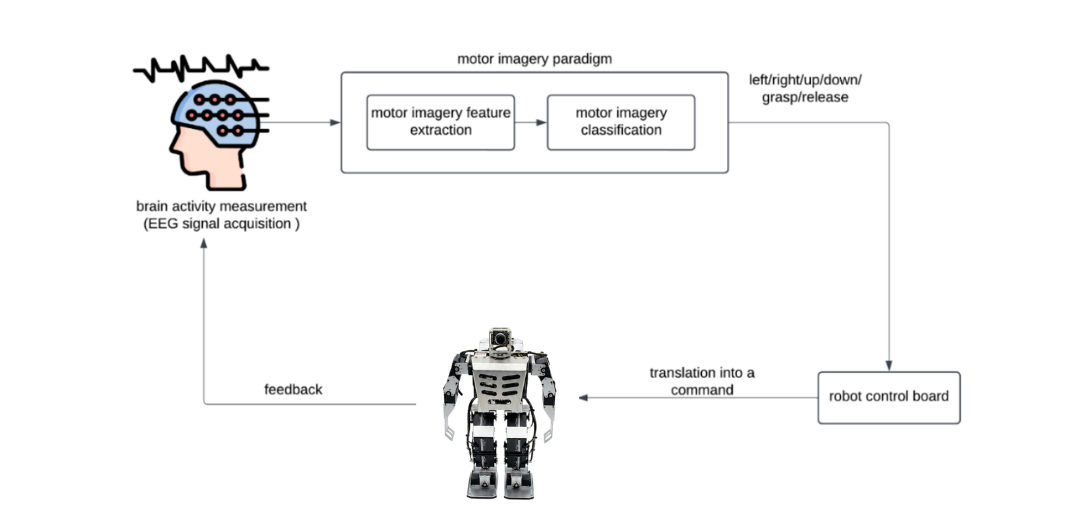
\includegraphics[width=0.80\textwidth]{fig_overview}
\caption{High-level overview of the NeuroMotion BCI pipeline. Brain activity is
measured via EEG, processed through the motor imagery feature extraction and
classification stages, and translated into directional commands that drive the
HBE Robonova AI3 humanoid robot. Physical robot motion provides closed-loop
feedback to the user.}
\label{fig:overview}
\end{figure}

\section{Literature Review}

A systematic review of recent literature (2019--2025) was conducted across IEEE Xplore,
PubMed, ACM Digital Library, and Google Scholar using the keywords: EEG,
brain--computer interface, motor imagery, robotic control.

\subsection{Signal Processing}

Bandpass filtering (8--30\,Hz) and Independent Component Analysis (ICA) are widely adopted
for noise and artifact reduction in EEG-based BCI systems \cite{mohamed2024}. The
Mu (8--12\,Hz) and Beta (13--30\,Hz) rhythms are the primary neural correlates of motor
imagery and form the frequency band of interest throughout this project.

\subsection{Feature Extraction}

Power Spectral Density (PSD) and wavelet transforms have demonstrated strong discriminatory
capability for EEG-based motor imagery classification \cite{elshahat2025}. Common Spatial
Patterns (CSP) effectively isolate spatially distinct features across EEG channels and are
particularly well-suited to binary motor imagery tasks, making them the feature extraction
method of choice for this system.

\subsection{Classification}

CNN-based models achieve over 90\% accuracy on benchmark motor imagery datasets.
However, for real-time deployment on resource-constrained systems, SVM with RBF kernel
provides the best balance of accuracy and computational efficiency \cite{cortes1995}.
LSTM and GRU networks improve classification by capturing temporal dependencies in EEG
sequences but introduce latency that conflicts with real-time actuation constraints.

\subsection{Gap Analysis}

Existing BCI systems for robotic control suffer from four recurring shortcomings:

\begin{enumerate}
    \item Limited portability and complex calibration procedures.
    \item Poor multi-class accuracy ($\geq$4 commands) due to spatial signal overlap.
    \item Absence of safety mechanisms for real-world deployment.
    \item Lack of security for transmitted neural data.
\end{enumerate}

NeuroMotion directly addresses all four gaps through its hierarchical classification
architecture, confidence gating, emergency stop system, and AES Fernet encryption.

\section{Background}

According to the WHO, over one billion people worldwide live with some form of disability,
of whom 75+ million require mobility assistance devices \cite{who2023}. An estimated
5.4 million people live with paralysis \cite{nscisc2021}. In developing regions, access to
assistive technology remains below 10\%. The growing demand for affordable, AI-enabled
assistive devices, combined with increased research interest in BCI technology, creates a
clear opportunity for systems like NeuroMotion.

Key concepts underpinning the project:

\begin{description}
    \item[EEG (Electroencephalography)] A non-invasive method of recording electrical
    brain activity through scalp-mounted sensors. EEG captures voltage fluctuations
    resulting from ionic current flows within neurons.

    \item[BCI (Brain-Computer Interface)] A direct communication pathway between the
    brain and an external device, bypassing conventional neuromuscular output channels.

    \item[Motor Imagery] The mental simulation of a physical movement without actual
    execution. Motor imagery is detectable as event-related synchronisation and
    desynchronisation in the Mu and Beta EEG frequency bands.

    \item[CSP (Common Spatial Patterns)] A spatial filtering algorithm that computes a
    projection matrix maximising the variance of one EEG class while simultaneously
    minimising the variance of the opposing class, producing discriminative features for
    binary classification.
\end{description}

\section{Functional and Non-Functional Requirements}

To realize the goal of a universally accessible and safe robotic control system, the engineering design of NeuroMotion is guided by a formal set of requirements. These requirements ensure that the system is both functionally complete and meets the high standards of performance, security, and safety necessary for real-world assistive technology.

\subsection{Functional Requirements}

Functional requirements define the core behaviors and operations that the NeuroMotion system must perform:

\begin{itemize}
    \item \textbf{Real-Time EEG Acquisition:} The system must connect to the wireless EEG headset and read real-time neural signals continuously during a session.
    \item \textbf{Signal Preprocessing:} The software must automatically filter, normalize, and remove artifacts from the raw EEG streams to isolate sensorimotor rhythms (Mu and Beta bands) without manual intervention.
    \item \textbf{Command Prediction:} The AI classifier must process the extracted feature vectors and predict the user's intended directional command (Forward, Backward, Left, Right, or Idle).
    \item \textbf{Hardware Command Dispatch:} The system must translate predicted commands into specific robotic instructions and transmit them to the HBE Robonova AI3 over a Serial/UART or Bluetooth communication interface.
    \item \textbf{Telemetry and Data Logging:} The system must log all raw/processed EEG segments, predicted labels, and execution timestamps for future retraining, calibration verification, and debugging.
    \item \textbf{Multi-Modal Control and Gaze Tracking:} The system must support an alternative webcam-based eye-tracking mode, processing video frames to predict eye gaze directions and mapping them to robot movements.
    \item \textbf{Safety Fail-Safes and Overrides:}
    \begin{itemize}
        \item The system must immediately issue a \texttt{STOP} command if a loss of EEG signal or WebSocket disconnection is detected.
        \item A manual override option must be available at all times in the GUI to allow an administrator or caregiver to stop or command the robot manually.
        \item Low-confidence predictions (below the threshold) must be automatically gated and defaulted to an \texttt{IDLE} or \texttt{STOP} action to prevent erroneous movement.
    \end{itemize}
\end{itemize}

\subsection{Non-Functional Requirements}

Non-functional requirements define the quality attributes, operational limits, and constraints of the NeuroMotion platform:

\begin{itemize}
    \item \textbf{Accuracy:} The machine learning pipeline must achieve at least $85$--$90\%$ prediction accuracy under calibrated, subject-specific conditions to ensure reliable control.
    \item \textbf{Latency:} The end-to-end processing delay --- from raw signal arrival at the server to command dispatch to the robot --- must remain under $150$--$300$\,ms to ensure a responsive, real-time user experience.
    \item \textbf{Reliability:} The system must sustain continuous, uninterrupted real-time streaming and inference for at least $1$ hour.
    \item \textbf{Usability and Accessibility:} The web interface (\textit{NeuroMotion::LINK}) must be intuitive, require minimal technical training, and feature a subject-calibration sequence that takes no longer than $1$--$2$ minutes.
    \item \textbf{Safety and Compliance:} All commanded motions must respect the physical and mechanical limits of the Robonova AI3. In any state of communication failure, sensor noise, or inference ambiguity, the system must fail-safe to a stationary state.
    \item \textbf{Maintainability:} The architecture must be highly modular, allowing the AI classification models or preprocessing parameters to be updated or replaced without modifying the web server or hardware control layers.
    \item \textbf{Scalability:} The software design and command mapping protocols must easily scale to support additional mental commands (such as vertical lifting, diagonal movements, or speed adjustments) in future releases.
    \item \textbf{Resource Constraints:} CPU and memory utilization on the host workstation must remain below $70\%$ during real-time streaming to prevent latency jitter.
    \item \textbf{Security:} All recorded sessions, user training sets, and telemetry databases must be securely stored and encrypted (using AES Fernet), with API endpoints protected by session tokens and access-control checks.
\end{itemize}

\section{Summary}

This chapter established the motivation, problem space, literature context, and foundational
concepts behind NeuroMotion. The full pipeline --- raw EEG preprocessing, CSP feature
extraction, hierarchical dual-SVM classification, confidence gating, and robot command
dispatch --- was implemented and validated in simulation using EEG motor imagery data
provided by Benha University. The following chapter presents the methodology, system
architecture, and design decisions that translate these requirements into a working system.

% ─────────────────────────────────────────────────────────────
%  CHAPTER 2 — Neuroscience Background & Hardware Platforms
% ─────────────────────────────────────────────────────────────
\chapter{Neuroscience Background \& Hardware Platforms}

This chapter provides the foundational knowledge necessary to understand how
NeuroMotion captures, interprets, and acts upon brain signals. It covers the
cellular origin of EEG signals, the functional organisation of the brain, the
principles of EEG recording, the oscillatory rhythms that underpin motor imagery,
artifact sources and their management, and the technical specification of the
headset used to acquire the dataset on which NeuroMotion was developed and validated.

% ─────────────────────────────────────────────────────────────
\section{Neurons and the Cellular Origin of EEG}
% ─────────────────────────────────────────────────────────────

The fundamental computational unit of the brain is the \textbf{neuron}, a
specialised electrochemical cell that receives, integrates, and transmits
information. Each neuron consists of three main structural components
(Figure~\ref{fig:neuron}):

\begin{figure}[!htbp]
\centering
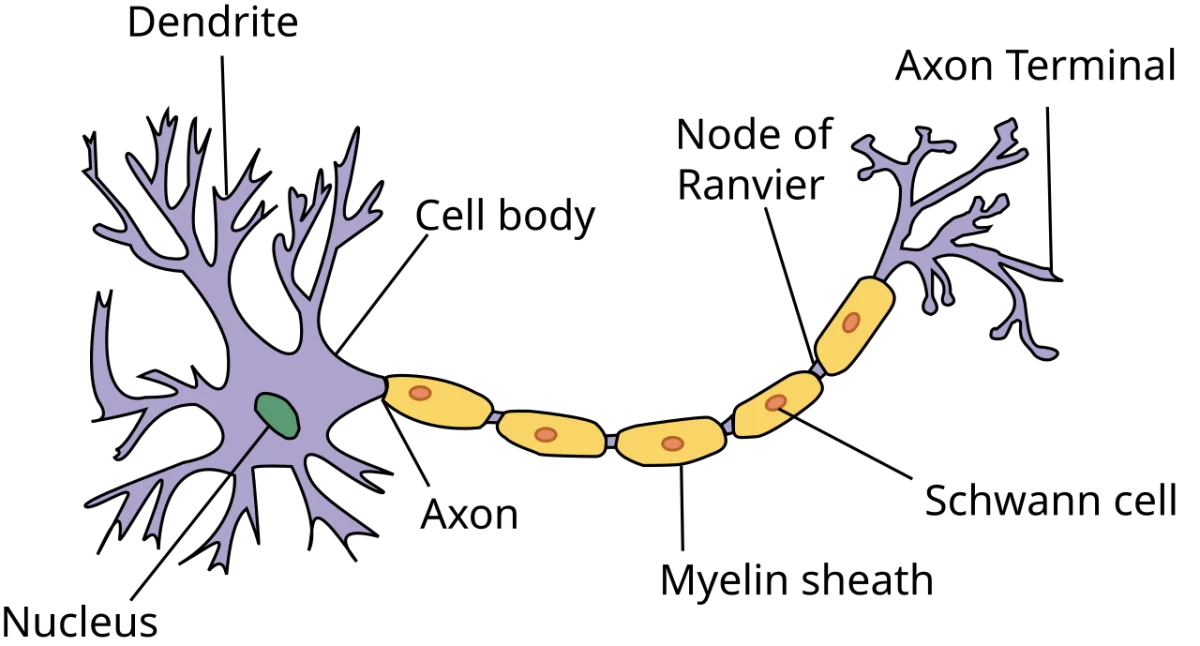
\includegraphics[width=0.70\textwidth]{fig_neuron}
\caption{Simplified schematic of a neuron showing dendrites, the cell body
(soma) containing the nucleus, the myelinated axon, and axon terminals.
EEG signals reflect the summated post-synaptic potentials of large
populations of cortical neurons rather than individual action potentials.}
\label{fig:neuron}
\end{figure}

\begin{itemize}
  \item \textbf{Dendrites:} Branch-like extensions that receive incoming signals
        from neighbouring neurons.
  \item \textbf{Cell Body (Soma):} Integrates incoming signals and contains the
        nucleus.
  \item \textbf{Axon:} A long, cable-like projection that transmits the neuron's
        output signal to other neurons, muscles, or glands. Many axons are
        insulated by a myelin sheath that accelerates signal propagation.
\end{itemize}

Neurons communicate at specialised junctions called \textbf{synapses}. When an
arriving electrical impulse (an \textit{action potential}) reaches the axon
terminal, it triggers the release of neurotransmitters into the synaptic cleft.
These bind to receptors on the adjacent neuron and alter its membrane potential.
When this cumulative input exceeds a threshold, the postsynaptic neuron fires its
own action potential --- a rapid, all-or-nothing depolarisation of the membrane from
approximately $-70$\,mV to a brief positive peak, followed by repolarisation.

\textbf{EEG signals do not directly reflect individual action potentials.} Rather,
they capture the \textit{summated post-synaptic potentials} of thousands to millions
of cortical pyramidal neurons firing in synchrony. Only when large populations of
spatially aligned neurons are co-activated simultaneously do their combined
electrical fields become detectable at the scalp surface \cite{nunez2006}.

% ─────────────────────────────────────────────────────────────
\section{The Brain and Motor Control}
% ─────────────────────────────────────────────────────────────

The human brain is the most complex organ in the body, comprising approximately
100 billion neurons interconnected by an estimated 500 trillion synapses. It is
divided into three primary structures: the \textbf{cerebrum}, the
\textbf{cerebellum}, and the \textbf{brain stem}. The cerebrum --- the largest
structure --- is covered by the cerebral cortex, a thin sheet of grey matter
organised into four lobes, each governing a distinct functional domain
(Figure~\ref{fig:brain_lobes}).

\begin{figure}[!htbp]
\centering
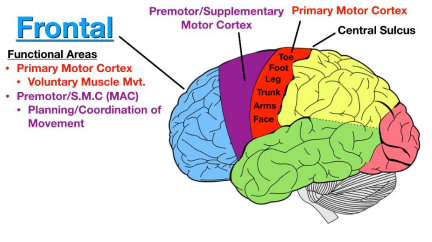
\includegraphics[width=0.65\textwidth]{fig_brain_lobes}
\caption{Schematic lateral view of the cerebral cortex showing the four lobes and
the motor cortex location along the central sulcus. The frontal lobe houses
the primary motor cortex and premotor areas most relevant to motor imagery-based BCIs.}
\label{fig:brain_lobes}
\end{figure}

The four lobes and their primary roles are:

\begin{itemize}
  \item \textbf{Frontal Lobe:} Governs executive functions, decision-making, language
        production, and --- critically for this project --- voluntary motor control via
        the primary motor cortex (M1) and the adjacent premotor and supplementary motor
        areas (SMA). These regions are responsible for planning, initiating, and
        coordinating voluntary movements.
  \item \textbf{Parietal Lobe:} Processes somatosensory information including touch,
        pressure, and spatial orientation.
  \item \textbf{Temporal Lobe:} Handles auditory processing, memory consolidation, and
        language comprehension.
  \item \textbf{Occipital Lobe:} Dedicated primarily to visual processing.
\end{itemize}

Of particular relevance to NeuroMotion is the \textbf{motor cortex and the
premotor/supplementary motor area}. During motor imagery --- the deliberate mental
simulation of a movement without physical execution --- these cortical regions
generate detectable patterns of electrical activity that closely resemble those
observed during actual movement, albeit at lower amplitude. This overlap forms the
neurophysiological basis for motor imagery BCI control \cite{pfurtscheller2001}.

% ─────────────────────────────────────────────────────────────
\section{Electroencephalography (EEG)}
% ─────────────────────────────────────────────────────────────

\subsection{Principles of Signal Generation and Transmission}

Electroencephalography (EEG) is a non-invasive neuroimaging modality that records
the brain's electrical activity as voltage fluctuations at the scalp surface. These
signals originate from the movement of ions (Na\textsuperscript{+},
K\textsuperscript{+}, Ca\textsuperscript{2+}, Cl\textsuperscript{-}) across
neuronal membranes, generating extracellular current flow detectable by surface
electrodes. Before reaching the electrodes, these signals propagate through multiple
tissue layers --- brain tissue, cerebrospinal fluid, the skull, and the scalp ---
each with a different electrical resistivity. The skull in particular has high
resistivity relative to brain tissue, substantially attenuating and spatially
smearing the signal. As a result, EEG has relatively coarse spatial resolution but
excellent temporal resolution (millisecond scale), making it well suited for
detecting the rapid oscillatory patterns associated with motor imagery.

\subsection{Recording Hardware and Digitisation}

Modern EEG systems amplify the microvolt-range scalp potentials using
high-gain differential amplifiers, then digitise the analog signals through
multi-channel analog-to-digital converters (ADCs). EEG bandwidth of physiological
interest extends to approximately 100\,Hz, so sampling rates of 128--2048 samples
per second are standard depending on the application. Signal conditioning prior to
analysis involves three standard filtering stages:

\begin{itemize}
  \item \textbf{High-pass filtering} (typically $>0.5$\,Hz): removes slow
        baseline drift caused by electrode impedance changes, electrode movement,
        or sweat.
  \item \textbf{Low-pass filtering} (typically $<50$--$70$\,Hz): attenuates
        high-frequency muscle noise and other broadband contamination above the
        range of neural interest.
  \item \textbf{Notch filtering at 50\,Hz} (60\,Hz in some regions): suppresses
        power-line electromagnetic interference, which is a dominant environmental
        artifact in any EEG recording.
\end{itemize}

\subsection{Electrode Placement: The 10--20 System}

The internationally standardised \textbf{10--20 electrode placement system}
specifies electrode positions as fixed percentages (10\% or 20\%) of the
anterior-posterior and lateral skull dimensions, measured from anatomical
landmarks: the nasion, inion, and preauricular points (Figure~\ref{fig:1020}).
This standardisation ensures that electrode positions are reproducible across
subjects and comparable across studies.

Electrodes are labelled by brain region (Fp~=~frontal pole, F~=~frontal,
C~=~central, P~=~parietal, O~=~occipital, T~=~temporal) with odd numbers
for left-hemisphere and even numbers for right-hemisphere sites. The central
electrodes C3 and C4 --- positioned directly over the left and right primary
motor cortices respectively --- are the most informative channels for
sensorimotor rhythm analysis and motor imagery classification.

\begin{figure}[!htbp]
\centering
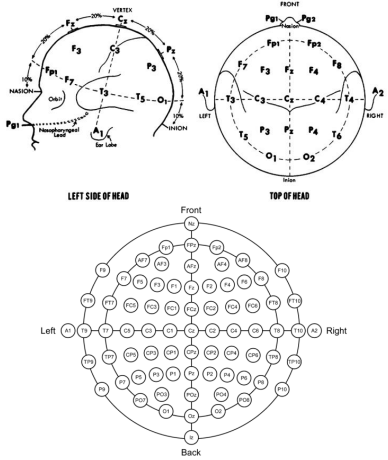
\includegraphics[width=0.55\textwidth]{fig_1020}
\caption{Top-view schematic of the 10--20 electrode placement system. C3 and C4
sit directly above the left and right primary motor cortices respectively.
The 14 channels of the Emotiv EPOC X used for dataset acquisition are highlighted.
Note that the EPOC X does not include C3/C4 directly; the acquisition team
repositioned the headset so that F3 and F4 approximated these locations.}
\label{fig:1020}
\end{figure}

% ─────────────────────────────────────────────────────────────
\section{Brain Rhythms and Sensorimotor Oscillations}
% ─────────────────────────────────────────────────────────────

EEG captures a continuous spectrum of oscillatory activity. This spectrum is
conventionally divided into frequency bands, each associated with distinct
cognitive and physiological states (Table~\ref{tab:brainrhythms}).

\begin{table}[h]
\centering
\caption{EEG frequency bands and their primary functional associations.}
\label{tab:brainrhythms}
\begin{tabular}{llp{7cm}}
\toprule
\textbf{Band} & \textbf{Range (Hz)} & \textbf{Primary Association} \\
\midrule
Delta ($\delta$) & 0.5 -- 4   & Deep sleep, slow-wave activity \\
Theta ($\theta$) & 4 -- 8     & Light sleep, relaxation, memory encoding \\
Alpha ($\alpha$) & 8 -- 13    & Relaxed wakefulness; eyes-closed resting state \\
Beta ($\beta$)   & 13 -- 30   & Active cognition, motor planning, focused attention \\
Gamma ($\gamma$) & 30 -- 100  & High-level cognitive processing, sensory binding \\
\midrule
Mu ($\mu$)       & 8 -- 12    & Sensorimotor rhythm; desynchronises during MI \\
\bottomrule
\end{tabular}
\end{table}

\subsection{The Mu and Beta Rhythms: Foundation of Motor Imagery BCI}

Of particular importance to NeuroMotion are the \textbf{Mu rhythm} (8--12\,Hz)
and the \textbf{Beta rhythm} (13--30\,Hz), both generated by the sensorimotor
cortex. These rhythms exhibit two characteristic modulations during motor activity
or motor imagery (Figure~\ref{fig:erd_ers}):

\begin{itemize}
  \item \textbf{Event-Related Desynchronization (ERD):} A decrease in oscillatory
        power in the Mu and Beta bands, occurring during or in anticipation of
        movement or motor imagery. ERD reflects an increase in cortical
        excitability and active neural processing --- the cortex is ``busy.''
  \item \textbf{Event-Related Synchronization (ERS):} A rebound increase in
        Beta-band power that typically follows movement cessation, reflecting
        cortical inhibition and motor disengagement.
\end{itemize}

Crucially, ERD and ERS are \textbf{lateralised}: imagining a left-hand movement
preferentially desynchronises the \textit{right} sensorimotor cortex (C4 region),
while imagining a right-hand movement desynchronises the \textit{left}
sensorimotor cortex (C3 region). This spatial asymmetry is the core discriminative
signal exploited by the CSP algorithm in the NeuroMotion classification pipeline
\cite{pfurtscheller1999}.

\begin{figure}[!htbp]
\centering
\includegraphics[width=0.70\textwidth]{fig_erd_ers}
\caption{Illustration of Event-Related Desynchronization (ERD) and
Event-Related Synchronization (ERS) during left-hand motor imagery. Relative
Mu/Beta band power at the contralateral motor cortex (C4) drops substantially
during the imagery period while the ipsilateral cortex (C3) remains near
baseline. This lateralised ERD/ERS pattern is the primary neural discriminator
exploited by the NeuroMotion CSP pipeline.}
\label{fig:erd_ers}
\end{figure}

% ─────────────────────────────────────────────────────────────
\section{Artifacts in EEG Recordings}
\label{sec:artifacts}
% ─────────────────────────────────────────────────────────────

A fundamental challenge in any EEG-based BCI system is the presence of
\textbf{artifacts} --- unwanted signals that contaminate the recording and can
obscure genuine neural activity. Artifacts are broadly classified into two
categories \cite{teplan2002}:

\paragraph{Subject-Related Artifacts}
These originate from physiological sources within the body. The most significant
for BCI applications are:

\begin{itemize}
  \item \textbf{Ocular artifacts (EOG):} Eye blinks and saccadic eye movements
        generate large-amplitude, low-frequency voltage deflections particularly
        prominent at frontal electrodes (AF3, F7, F4, F8 in the EPOC X layout).
        These are among the most disruptive artifacts due to their large amplitude
        relative to cortical signals.
  \item \textbf{Muscular artifacts (EMG):} Contractions of facial, neck, or
        scalp muscles introduce broadband electrical activity --- especially above
        30\,Hz --- that can be mistaken for neural signal.
  \item \textbf{Cardiac artifacts (ECG):} The heartbeat generates rhythmic
        electrical pulses detectable at temporal electrodes.
  \item \textbf{Movement artifacts:} Head or body motion introduces large,
        transient voltage disturbances.
\end{itemize}

\paragraph{Technique-Related Artifacts}
These arise from the recording environment or equipment:

\begin{itemize}
  \item \textbf{Power-line interference (50\,Hz):} Electromagnetic interference
        from mains electricity, suppressed by notch filtering.
  \item \textbf{Electrode impedance fluctuations:} Poor electrode-scalp contact,
        dried saline, or cable movement introduce noise or baseline drift.
  \item \textbf{Amplifier saturation:} Excessively large input voltages cause
        signal clipping.
\end{itemize}

Artifact management strategy depends on the artifact type. Large, transient
artifacts (e.g., body movements) are typically addressed by
\textbf{epoch rejection} --- discarding the contaminated trial entirely.
Persistent lower-amplitude artifacts such as ocular and cardiac signals are
handled more effectively through \textbf{Independent Component Analysis (ICA)},
a blind source separation technique that decomposes the multi-channel EEG into
statistically independent components, allowing artifact sources to be identified
and removed without discarding entire trials. The specific artifact handling
strategy applied to the NeuroMotion dataset is described in
Chapter~\ref{ch:signal_processing}.

% ─────────────────────────────────────────────────────────────
\section{The Emotiv EPOC X EEG Headset}
\label{sec:epocx}
% ─────────────────────────────────────────────────────────────

The EEG dataset underlying NeuroMotion was acquired by the Benha University
research team (Eng.\ Heba Maher El-Shahat et al.) using the
\textbf{Emotiv EPOC X} headset \cite{emotiv2024}. The EPOC X is a consumer-grade,
research-capable wireless EEG device combining portability with sufficient signal
quality for motor imagery BCI research. Due to logistical constraints that
prevented the NeuroMotion team from obtaining the hardware directly, the
pre-recorded dataset generously shared by the Benha team was used as the
experimental data foundation for all preprocessing, feature extraction,
classification, and system validation work described in this report.

The key technical specifications of the EPOC X are:

\begin{table}[h]
\centering
\caption{Emotiv EPOC X technical specifications.}
\label{tab:epocx}
\begin{tabular}{ll}
\toprule
\textbf{Parameter} & \textbf{Specification} \\
\midrule
EEG channels & 14 (AF3, F7, F3, FC5, T7, P7, O1, O2, P8, T8, FC6, F4, F8, AF4) \\
Reference electrodes & CMS/DRL (behind ears) \\
Electrode type & Saline-based Ag/AgCl sensors \\
Sampling rate & 128 or 256\,Hz (internal clock at 2048\,Hz) \\
Resolution & 14-bit (adjustable to 16-bit) \\
Bandwidth & 0.2 -- 45\,Hz (5th-order Sinc filter) \\
Notch filters & 50\,Hz and 60\,Hz (digital) \\
Connectivity & 2.4\,GHz wireless / Bluetooth LE / USB \\
Battery life & Up to 9 hours (lithium polymer) \\
Impedance monitoring & Real-time contact quality feedback \\
\bottomrule
\end{tabular}
\end{table}

\begin{figure}[!htbp]
\centering
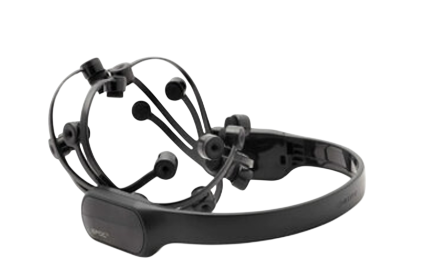
\includegraphics[width=0.60\textwidth]{fig_epoc_x}
\caption{The Emotiv EPOC X wireless EEG headset used for data acquisition by the
Benha University research team. The 14 saline-based Ag/AgCl electrodes are arranged
along the frontal, temporal, parietal, and occipital regions. The two reference
electrodes (CMS/DRL) are located behind the ears. Wireless transmission via 2.4\,GHz
or Bluetooth LE enables unrestricted movement during recording sessions.}
\label{fig:epoc_x}
\end{figure}

A notable hardware constraint relevant to NeuroMotion is that the EPOC X does not
include electrodes at the standard C3 and C4 positions, which are optimal for
recording sensorimotor activity. The Benha acquisition team addressed this by
carefully repositioning the headset so that electrodes F3 and F4 approximated the
C3 and C4 locations respectively, improving coverage of the motor cortex while
preserving data quality across the frontal, temporal, and parietal regions
\cite{elshahat2025}.

% ─────────────────────────────────────────────────────────────
\section{The HBE Robonova AI3 Humanoid Robot}
\label{sec:robonova}
% ─────────────────────────────────────────────────────────────

The target actuation platform for NeuroMotion is the \textbf{HBE Robonova AI3}
(also referred to as the Robonova HBE~3), a compact bipedal humanoid robot
developed by HBE Co., Ltd. of South Korea \cite{hbe2024}. The Robonova AI3 is a
programmable research and education platform well suited to BCI integration
projects due to its straightforward serial command interface and its library of
pre-programmed motion primitives covering locomotion, turning, and complex
full-body actions.

\begin{figure}[!htbp]
\centering
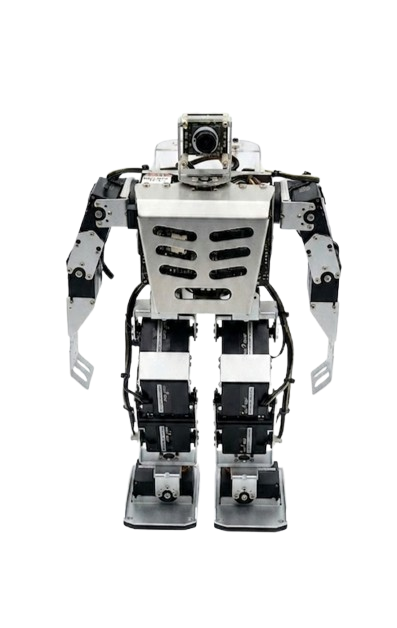
\includegraphics[width=0.45\textwidth]{fig_robonova}
\caption{The HBE Robonova AI3 humanoid robot --- the target actuation platform
for NeuroMotion. The robot accepts single-byte movement commands over a
Serial/UART connection at 4800\,baud, enabling real-time control from the
NeuroMotion backend inference engine.}
\label{fig:robonova}
\end{figure}

\subsection{Physical Characteristics}

The Robonova AI3 is a small-scale biped standing approximately 30\,cm tall and
weighing around 1\,kg. It is driven by 16 high-torque RC servo motors distributed
across the hip, knee, ankle, shoulder, and elbow joints, allowing it to execute a
rich repertoire of coordinated full-body motions. Its compact form factor makes it
practical for laboratory demonstrations and controlled environments typical of BCI
validation studies.

\subsection{Command Reception and Serial Interface}

The Robonova AI3 receives motion commands via a \textbf{Serial/UART interface}
operating at \textbf{4800\,baud} with an 8N1 frame format (8 data bits, no
parity, 1 stop bit). The robot's onboard motion controller listens continuously
on this serial port and interprets incoming data as \textbf{single unsigned byte
command codes}, each corresponding to one of its 32 pre-programmed motion
sequences (see Table~\ref{tab:robot_commands}).

Upon receiving a valid command byte, the Robonova AI3's onboard controller
immediately begins executing the corresponding motion primitive. No
acknowledgement packet is returned by the robot; the communication is therefore
strictly one-directional (host-to-robot). The NeuroMotion backend accounts for
this by enforcing a \textbf{1.5-second busy window} after each dispatch, during
which further commands are suppressed. This prevents a new command from
interrupting a motion sequence that is still in progress, which could otherwise
cause servo contention, unstable posture, or mechanical damage.

In the NeuroMotion system, the PySerial library manages the host-side serial
port (\texttt{COM8} by default on the deployment workstation). The four primary
directional commands used during BCI-driven control --- Forward, Backward, Left
Turn, and Right Turn --- map directly to command codes \texttt{FWD\_SHORT\_STEP}
(11), \texttt{BWD\_SHORT\_STEP} (12), \texttt{GO\_LEFT} (14), and
\texttt{GO\_RIGHT} (13) respectively. All 32 available command codes are
additionally exposed through the NeuroMotion::LINK manual override panel,
allowing an operator to send any motion primitive directly from the GUI
independent of the AI pipeline.

% ─────────────────────────────────────────────────────────────
\section{Summary}
% ─────────────────────────────────────────────────────────────

This chapter established the neurophysiological foundation of the NeuroMotion
system. The motor cortex and adjacent premotor areas generate detectable EEG
patterns during motor imagery, specifically ERD of the Mu and Beta sensorimotor
rhythms. These patterns are spatially lateralised --- left-hand imagery
desynchronises the right cortex and vice versa --- providing the discriminative
signal that CSP and SVM exploit. EEG recordings are contaminated by ocular,
muscular, and environmental artifacts that must be managed before classification.
The dataset used throughout this project was acquired using the Emotiv EPOC X by
the Benha University research team, whose hardware and protocol details have been
documented here as the basis for understanding all downstream processing decisions.

%% (Bibliography entries moved to the \begin{thebibliography} block at end of document)

% ─────────────────────────────────────────────────────────────
%  CHAPTER 3 — AI & Signal Processing Architecture
% ─────────────────────────────────────────────────────────────
\chapter{Artificial Intelligence \& Signal Processing Architecture}
\label{ch:signal_processing}

\section{Architecture Overview}

The core intelligence of the NeuroMotion system relies on a custom-engineered machine
learning pipeline designed for Brain-Computer Interface (BCI) execution. The pipeline is
divided into five distinct phases:

\begin{description}
    \item[Phase 1 --- Data Acquisition \& Preprocessing]
    Raw 14-channel EEG data is passed through a strict bandpass filter (8--30\,Hz),
    stripping baseline drift and high-frequency noise to focus entirely on the Mu
    (8--12\,Hz) and Beta (13--30\,Hz) sensorimotor rhythms. Zero-mean normalisation
    removes DC offset, and stimulus-locked temporal segmentation isolates 1.0-second
    epochs of active neural data.

    \item[Phase 2 --- Real-Time Artifact Rejection]
    To prevent Electrooculography (EOG) noise (e.g.\ eye blinks) from corrupting
    predictions, the pipeline monitors frontal channels (AF3, F7). If voltage exceeds a
    predefined physiological threshold, the affected frame is discarded and the system
    enters an \texttt{IDLE} state until a clean frame is available.

    \item[Phase 3 --- Spatial Feature Extraction]
    Common Spatial Patterns (CSP) translate the multi-channel EEG time-series into
    compact, discriminative feature vectors by maximising the variance ratio between
    opposing command classes, substantially improving the signal-to-noise ratio ahead
    of classification.

    \item[Phase 4 --- Hierarchical Classification]
    Rather than a single multi-class model, a divide-and-conquer ensemble of Support
    Vector Machines (SVM) was engineered. A \textbf{Horizontal Specialist} (Model~A)
    classifies Left vs.\ Right, and a \textbf{Vertical Specialist} (Model~B) classifies
    Forward vs.\ Backward. Both models run in parallel at inference time.

    \item[Phase 5 --- Decision Gating]
    Probabilistic gating (confidence $>$60\%) and temporal smoothing via a rolling
    frame buffer ensure that the robot command layer executes only on stable,
    high-confidence predictions, eliminating false positives caused by transient
    electrical artefacts.
\end{description}

\section{Model Benchmarking \& Architecture Justification}

To ensure operational reliability, rigorous benchmarking was conducted before finalising
the classification architecture. Both classical linear models and deep learning approaches
were evaluated.

\subsection{The Deep Learning Deficit}

Deep Convolutional Neural Networks (CNNs), specifically ResNet-inspired architectures,
were evaluated by transforming 1D EEG time-series into 2D spatial spectrograms.
The results were consistently worse in practice for three reasons:

\begin{enumerate}
    \item \textbf{Data hunger and overfitting:} CNNs require large training sets.
    On subject-specific calibration data of typical BCI scale, they rapidly memorised
    noise artefacts rather than genuine motor imagery patterns.

    \item \textbf{Inference latency:} The matrix multiplications required for deep
    inference violated the sub-1.5-second execution constraint imposed by the
    Robonova hardware interface.

    \item \textbf{Overconfidence:} Deep models assigned $>$95\% probability to
    random eye twitches, making the confidence gate ineffective as a safety mechanism.
\end{enumerate}

\subsection{The Linear Model Deficit}

Linear Discriminant Analysis (LDA) was also evaluated. LDA consistently underperformed
because it assumes linear separability in the feature space. Extracted CSP features
from EEG signals inherently occupy a non-linear, high-dimensional decision boundary
that LDA cannot adequately model.

\subsection{The Selected Solution: Hierarchical SVM with RBF Kernel}

The hierarchical dual-SVM architecture with RBF kernel provided the optimal engineering
trade-off across all criteria:

\begin{itemize}
    \item Successfully maps non-linear decision boundaries via the kernel trick.
    \item Requires minimal calibration data without overfitting.
    \item Maintains ultra-low inference latency suitable for real-time robotic actuation.
    \item Produces calibrated probability estimates via Platt Scaling, enabling effective
          confidence gating.
\end{itemize}

Table~\ref{tab:benchmarking} summarises the comparative benchmarking results.

\begin{table}[h]
\centering
\caption{Classifier Benchmarking Results}
\label{tab:benchmarking}
\begin{tabular}{lll}
\toprule
\textbf{Algorithm} & \textbf{Rank} & \textbf{Notes} \\
\midrule
SVM (RBF Kernel)  & 1st & Non-linear boundaries; optimal latency and accuracy \\
LDA               & 2nd & Fast but assumes linear separability; weaker on EEG \\
Random Forest     & 3rd & Good generalisation; higher computational cost \\
XGBoost           & 4th & Strong but slower to train and infer \\
KNN               & 5th & Distance-based; sensitive to noise and scaling \\
\bottomrule
\end{tabular}
\end{table}

\section{Mathematical Foundations \& Signal Processing}

\subsection{Signal Preprocessing \& Temporal Filtering}

To isolate the Sensorimotor Rhythms (SMR), a digital Butterworth bandpass filter is
applied across the 8--30\,Hz band. A zero-phase filtering technique (forward and backward
pass) is used to ensure that the temporal phase of EEG signals is not distorted during
processing, which is critical for preserving the timing of motor imagery events.

\subsection{Spatial Feature Extraction via CSP}

For a given single-trial EEG window $\mathbf{E}$ of dimensions $C \times T$
(Channels $\times$ Samples), the normalised spatial covariance matrix is computed as:

\begin{equation}
    \mathbf{\Sigma} = \frac{\mathbf{E}\mathbf{E}^{\top}}{\mathrm{tr}(\mathbf{E}\mathbf{E}^{\top})}
\end{equation}

For each binary specialist model, a composite covariance matrix is formed by averaging
across trials of the two opposing classes. Eigenvalue decomposition of this composite
matrix yields a projection matrix $\mathbf{W}$. The raw EEG trial is projected into a
new spatial subspace:

\begin{equation}
    \mathbf{Z} = \mathbf{W}^{\top} \mathbf{E}
\end{equation}

The variance of each projected signal is computed and log-transformed to produce the
final feature vector passed to the classifier:

\begin{equation}
    f_i = \log\left(\frac{\mathrm{var}(\mathbf{Z}_i)}{\sum_j \mathrm{var}(\mathbf{Z}_j)}\right)
\end{equation}

\subsection{Non-Linear Classification via SVM with RBF Kernel}

The SVM classifier finds the optimal separating hyperplane by solving a constrained
quadratic optimisation problem. The RBF kernel maps input features into a
higher-dimensional space to handle non-linear class boundaries:

\begin{equation}
    K(\mathbf{x}_i, \mathbf{x}_j) = \exp\left(-\gamma \|\mathbf{x}_i - \mathbf{x}_j\|^2\right)
\end{equation}

where $\gamma$ controls the sphere of influence of each training example.
The decision function is:

\begin{equation}
    f(\mathbf{x}) = \mathrm{sign}\left(\sum_{i} \alpha_i y_i K(\mathbf{x}_i, \mathbf{x}) + b\right)
\end{equation}

where $\alpha_i$ are the Lagrange multipliers, $y_i \in \{-1, +1\}$ are class labels,
and $b$ is the bias term. The margin between support vectors is maximised to ensure
the best generalisation to unseen EEG epochs.

\section{Hyperparameter Tuning \& Dataset Configuration}

\subsection{Epoch Window Size}

The continuous EEG stream is segmented into sliding windows of exactly 1.5 seconds.
This duration was selected as the optimal engineering trade-off: it provides a
sufficiently dense data matrix for CSP to compute stable covariance estimates, while
keeping total algorithmic processing time within the sub-1.5-second execution
constraint required for seamless real-time robot actuation.

\subsection{SVM Regularisation Parameter \textit{C}}

The penalty parameter $C$ governs the trade-off between maximising the margin and
minimising training error. It was tuned using Grid Search Cross-Validation to enforce
a soft margin, allowing the model to tolerate minor noisy outliers rather than
overfitting to them.

\subsection{Kernel Coefficient \texorpdfstring{$\gamma$}{gamma}}

The $\gamma$ parameter was scaled relative to the feature dimensionality
(\texttt{scale} heuristic) to define an appropriate sphere of influence per training
example, preventing the decision boundary from becoming excessively rigid or irregular.

\section{Probabilistic Gating \& Temporal Smoothing}

To meet the strict safety requirements of robotic actuation, the backend applies a
two-stage gating mechanism on top of the raw SVM output.

\textbf{Platt Scaling} converts the SVM's distance-to-boundary metric into a true class
probability estimate. A strict \textbf{60\% confidence threshold} is then enforced:
any prediction below this threshold is treated as uncertain and the system defaults to
\texttt{IDLE/STOP} rather than dispatching a movement command.

\textbf{Temporal Smoothing} further reinforces safety via a rolling frame buffer. The
robot command layer executes only when the buffer demonstrates consecutive prediction
agreement across multiple frames (configurable via \texttt{DEMO\_STREAK\_REQUIRED},
default: 2 consecutive frames). This eliminates false positives caused by transient
electrical spikes or single-frame misclassifications.

\section{Core Software Stack \& Dependencies}

\begin{table}[h]
\centering
\caption{Core Software Stack}
\label{tab:software_stack}
\begin{tabular}{ll}
\toprule
\textbf{Component} & \textbf{Library / Tool} \\
\midrule
EEG Signal Processing    & MNE-Python, SciPy (\texttt{butter}, \texttt{filtfilt}) \\
Feature Extraction       & scikit-learn (CSP), SciPy (\texttt{welch}), PyWavelets \\
AI / Classification      & scikit-learn (SVC, LDA, RandomForest, XGBoost, KNN) \\
Probabilistic Calibration & scikit-learn (\texttt{CalibratedClassifierCV} / Platt Scaling) \\
Backend API              & Flask, Python \texttt{cryptography} (AES Fernet) \\
Robot Communication      & PySerial (Serial/UART to Robonova AI3) \\
Numerical Computing      & NumPy \\
\bottomrule
\end{tabular}
\end{table}

\section{Summary}

This chapter presented the complete AI and signal processing architecture underpinning
NeuroMotion, from raw EEG preprocessing to final directional command generation. The
hierarchical dual-SVM design, justified by rigorous benchmarking against deep learning
and linear alternatives, provides a reliable, safe, and computationally efficient solution
for BCI-driven robotic control. The mathematical foundations --- Butterworth filtering,
CSP projection, RBF-SVM classification, and Platt-scaled confidence gating --- form a
coherent pipeline in which each stage is motivated by the specific constraints of
real-time EEG-based motor imagery decoding.

% ─────────────────────────────────────────────────────────────
%  CHAPTER 4 — System Implementation & Results
% ─────────────────────────────────────────────────────────────
\chapter{System Implementation \& Results}
\label{ch:implementation}

This chapter documents the concrete engineering decisions, implementation details, and
validation results of the NeuroMotion system. It bridges the algorithmic foundations
presented in Chapters 2 and 3 with the working software artefact delivered as the
project outcome. Each section describes a distinct component of the system architecture,
referencing specific source files, configuration parameters, and measured outcomes.

% ─────────────────────────────────────────────────────────────
\section{System Architecture Overview}
\label{sec:arch_overview}
% ─────────────────────────────────────────────────────────────

NeuroMotion follows a \textbf{three-tier client-server architecture} that separates
presentation, application logic, and hardware communication into independent layers
(see Figure~\ref{fig:overview} for a high-level pipeline overview).
This modular design allows individual components to be developed, tested, and replaced
independently, and enables multiple simultaneous clients to access the system over a
local network.

\begin{description}
    \item[Tier 1 --- Frontend (Presentation Layer)]
    The \textbf{NeuroMotion::LINK} web GUI is rendered by a Flask/Jinja2 templating
    engine and delivered to the client browser over HTTP. Real-time telemetry updates
    are fetched by JavaScript polling the REST API at configurable intervals. The
    interface requires no client-side installation, running in any modern browser on a
    local network connection.

    \item[Tier 2 --- Backend (Application Layer)]
    Two co-deployed Python servers form the application layer:
    \begin{itemize}
      \item A \textbf{Flask application} (port 5000) handles authentication, session
            management, the EEG demo engine, and REST API endpoints for the GUI.
      \item A \textbf{FastAPI application} (port 8000) hosts the eye tracking
            inference service, receiving webcam frames over WebSocket and returning
            real-time gaze direction predictions.
    \end{itemize}

    \item[Tier 3 --- Hardware (Communication Layer)]
    All robot commands are serialised as single-byte codes and transmitted over
    PySerial (Serial/UART) at 4800\,baud to the HBE Robonova AI3 on COM8. A
    thread-safe lock and 1.5-second busy window prevent command collision.

\begin{figure}[!htbp]
\centering
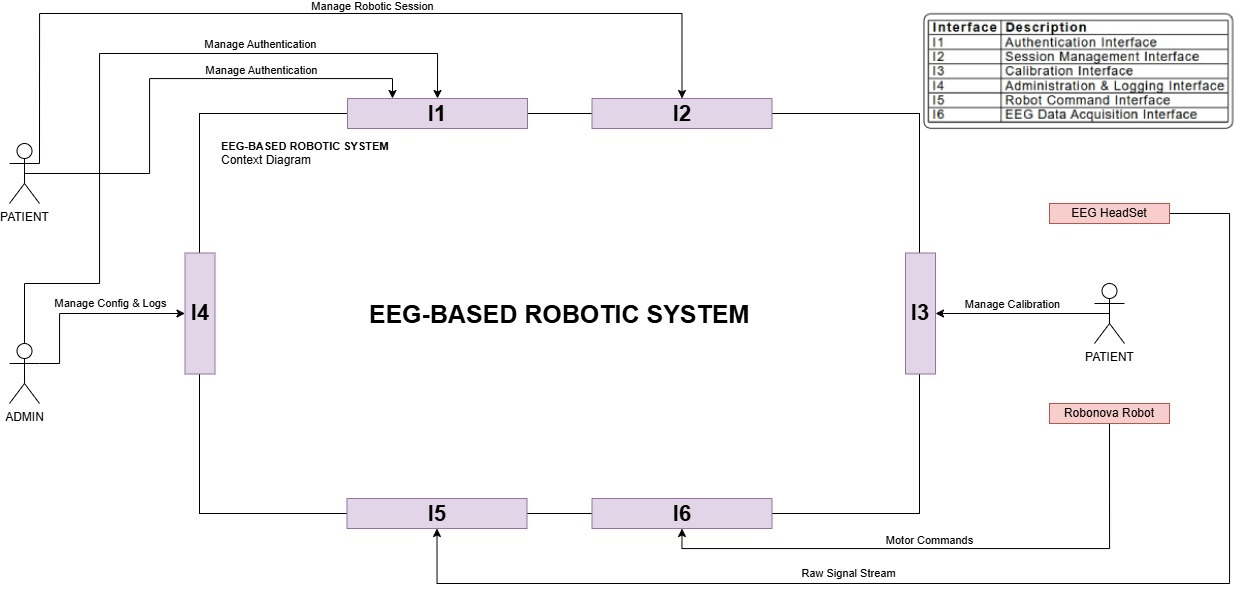
\includegraphics[width=0.75\textwidth]{fig_system_architecture.jpg.jpeg}
\caption{High-level system architecture of NeuroMotion. The three-tier design
separates the Flask/Jinja2 GUI frontend, the Python dual-server application layer
(EEG demo engine + eye tracking FastAPI service), and the PySerial hardware
communication layer to the Robonova AI3 robot.}
\label{fig:system_architecture}
\end{figure}
\FloatBarrier

% ─────────────────────────────────────────────────────────────
\section{Software Design Diagrams}
\label{sec:design_diagrams}
% ─────────────────────────────────────────────────────────────

This section presents the standard UML and structured analysis diagrams produced
during the design phase of NeuroMotion. Together they provide a comprehensive
view of system behaviour, component responsibilities, data flow, and state
management from multiple complementary perspectives.

\subsection{Use Case Diagram}

The Use Case diagram in Figure~\ref{fig:use_case} captures the interactions
between the two primary actors --- the \textbf{User} (operator with motor
disability) and the \textbf{Administrator} --- and the functional capabilities
exposed by the system. Key use cases include initiating an EEG session, issuing
mental commands, activating eye tracking mode, viewing session telemetry,
performing manual override, and managing user accounts.

\begin{figure}[!htbp]
\centering
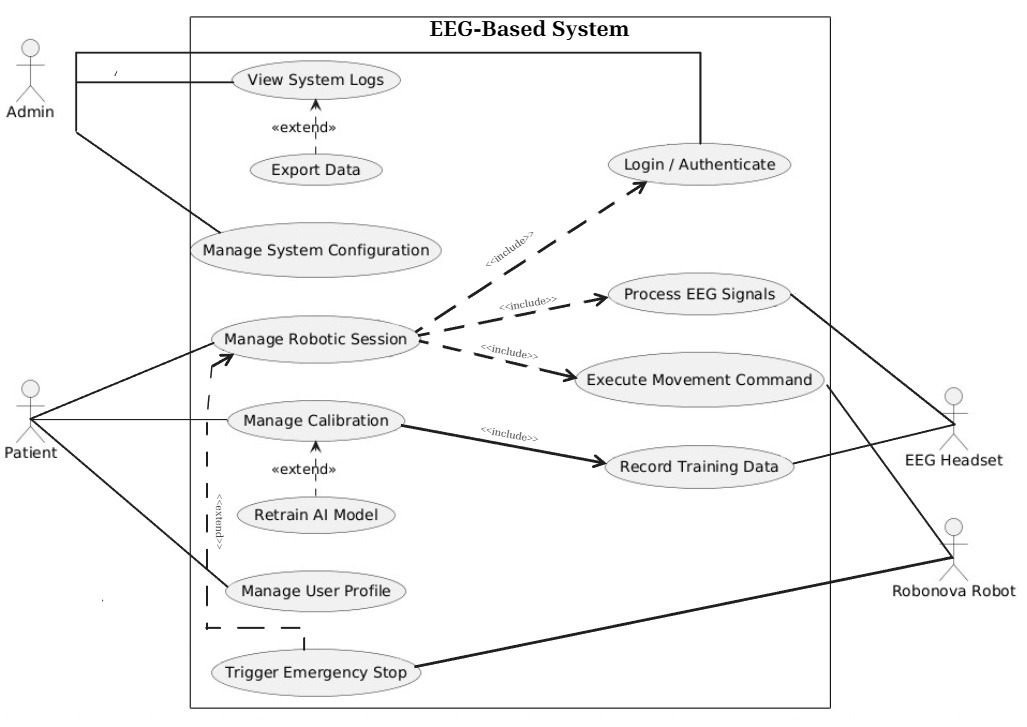
\includegraphics[width=0.75\textwidth]{Use Case}
\caption{Use Case diagram for the NeuroMotion system. The User actor interacts
with the core BCI control and monitoring functions, while the Administrator
additionally manages user accounts and system configuration.}
\label{fig:use_case}
\end{figure}
\FloatBarrier

\subsection{Sequence Diagram}

Figure~\ref{fig:sequence_diagram} traces the temporal message flow for a
complete EEG-driven command cycle: from the user initiating a streaming session
through EEG acquisition and inference to the final robot command dispatch and
GUI update. The diagram highlights the interactions between the browser client,
Flask backend, EEG demo engine, inference controller, and the Robonova AI3 serial
interface.

\begin{figure}[!htbp]
\centering
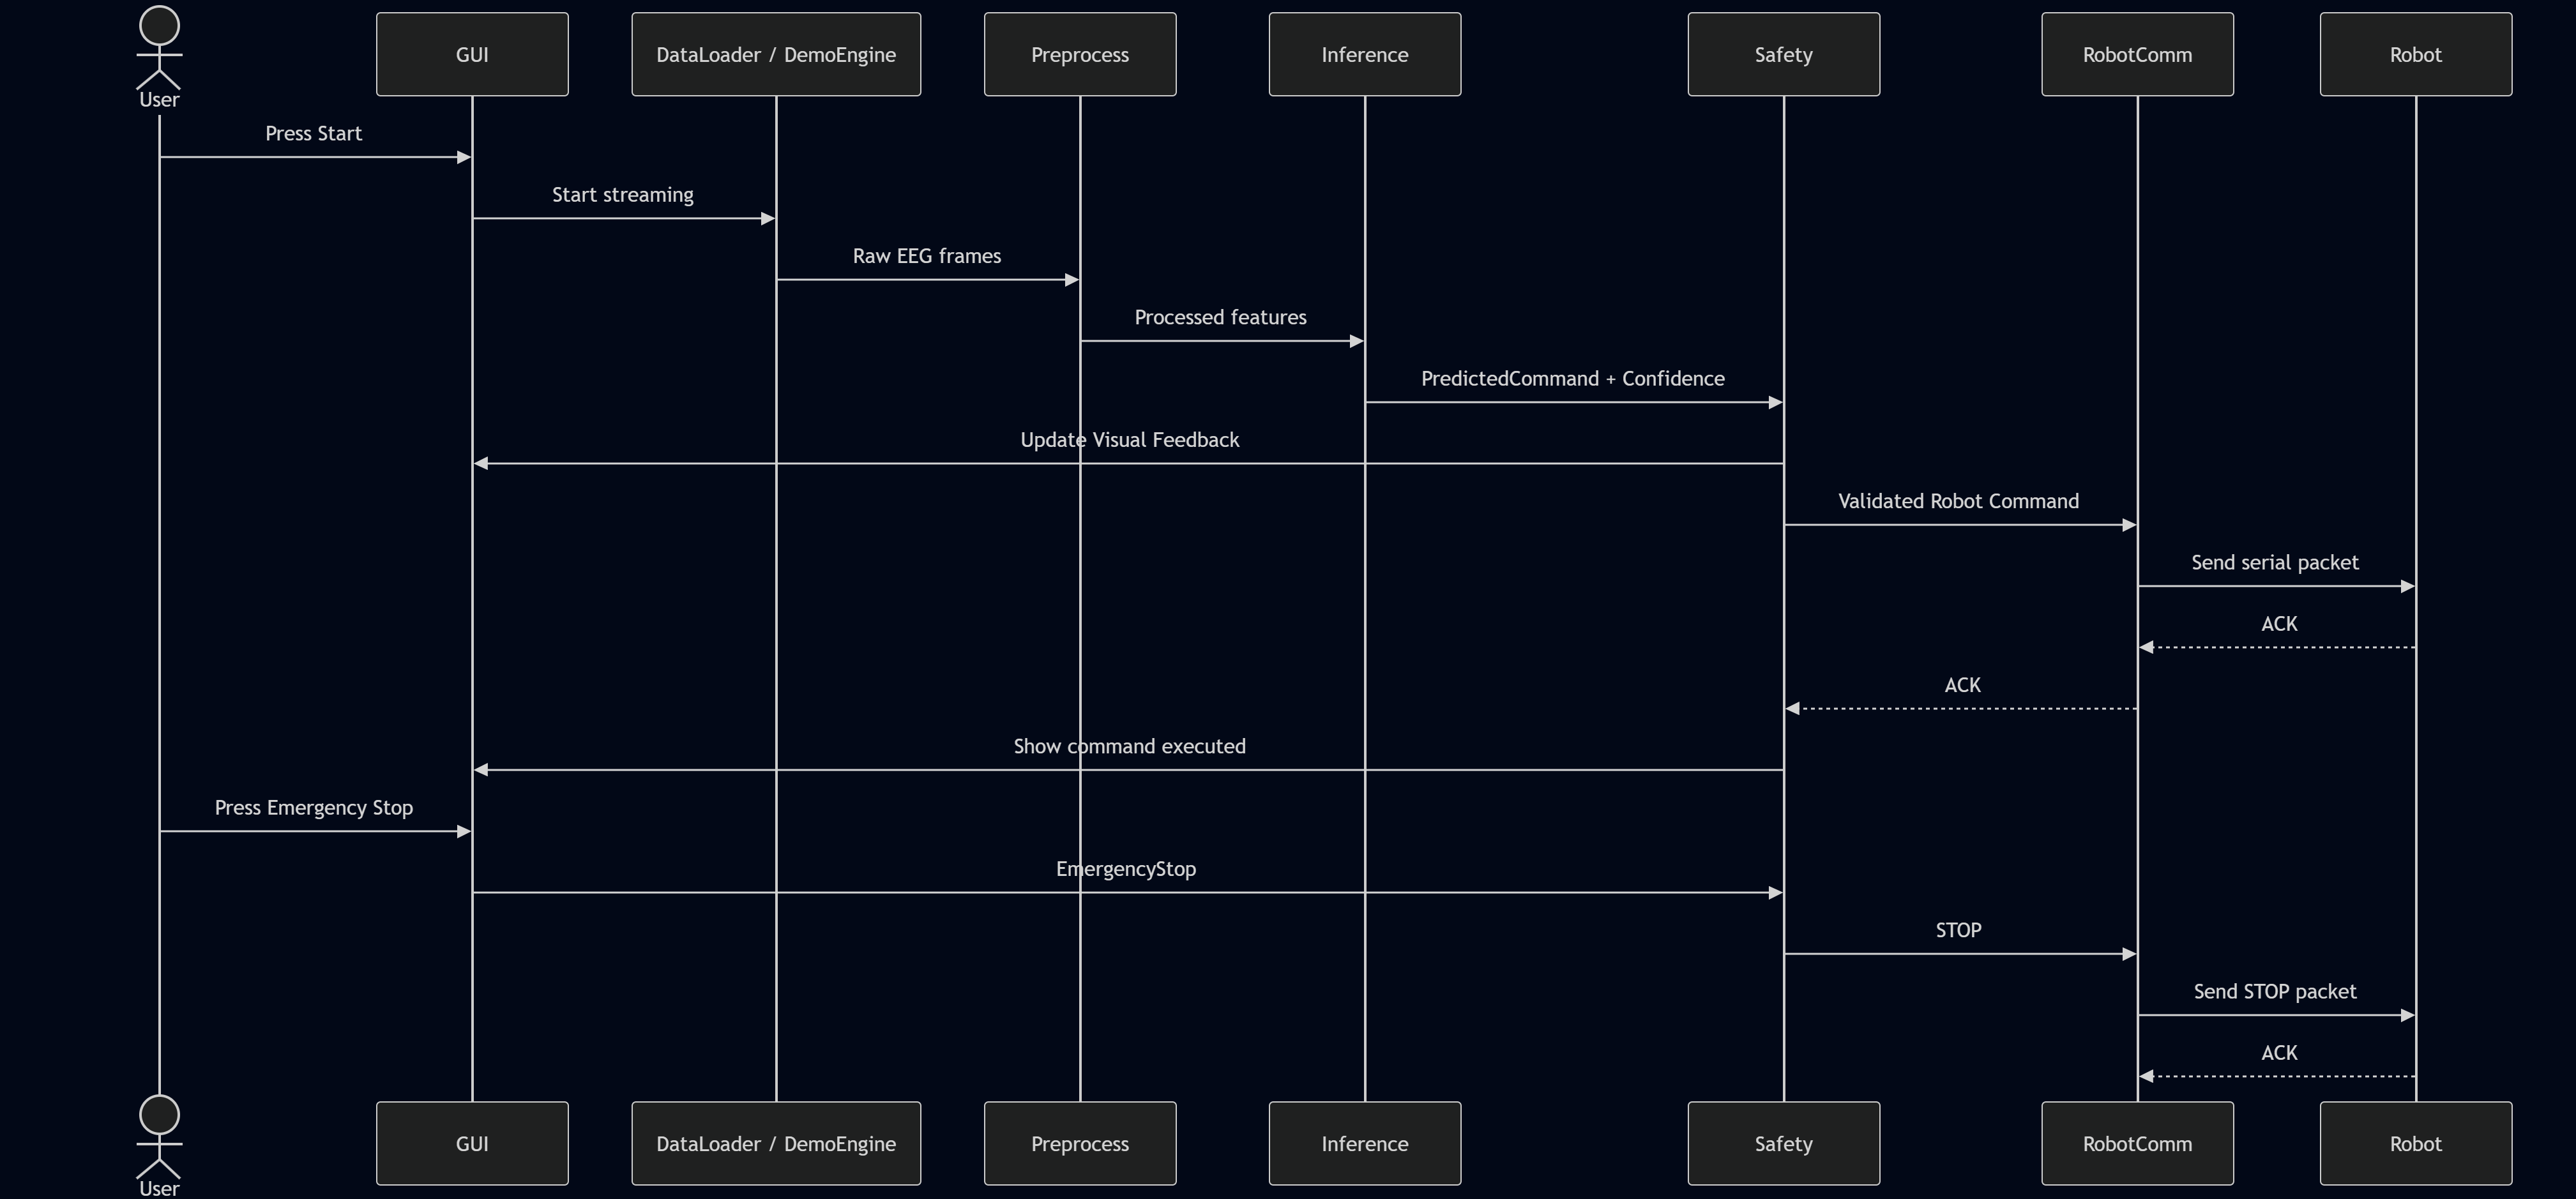
\includegraphics[width=0.80\textwidth]{Sequence-Diagram}
\caption{Sequence diagram for an EEG mental command cycle in NeuroMotion. The
message flow proceeds from session start through preprocessing, CSP feature
extraction, hierarchical SVM inference, confidence gating, and serial command
dispatch, returning telemetry to the GUI on each frame.}
\label{fig:sequence_diagram}
\end{figure}
\FloatBarrier

\subsection{Component Diagram}

The Component diagram (Figure~\ref{fig:component_diagram}) depicts the major
software components of the NeuroMotion system and their dependency relationships.
Primary components include the Flask Web Application, EEG Demo Engine, Inference
Controller, Eye Tracking FastAPI Service, Security Vault, and the SQLite
persistence layer. The diagram makes explicit which components communicate over
HTTP, WebSocket, PySerial, and internal Python function calls.

\begin{figure}[!htbp]
\centering
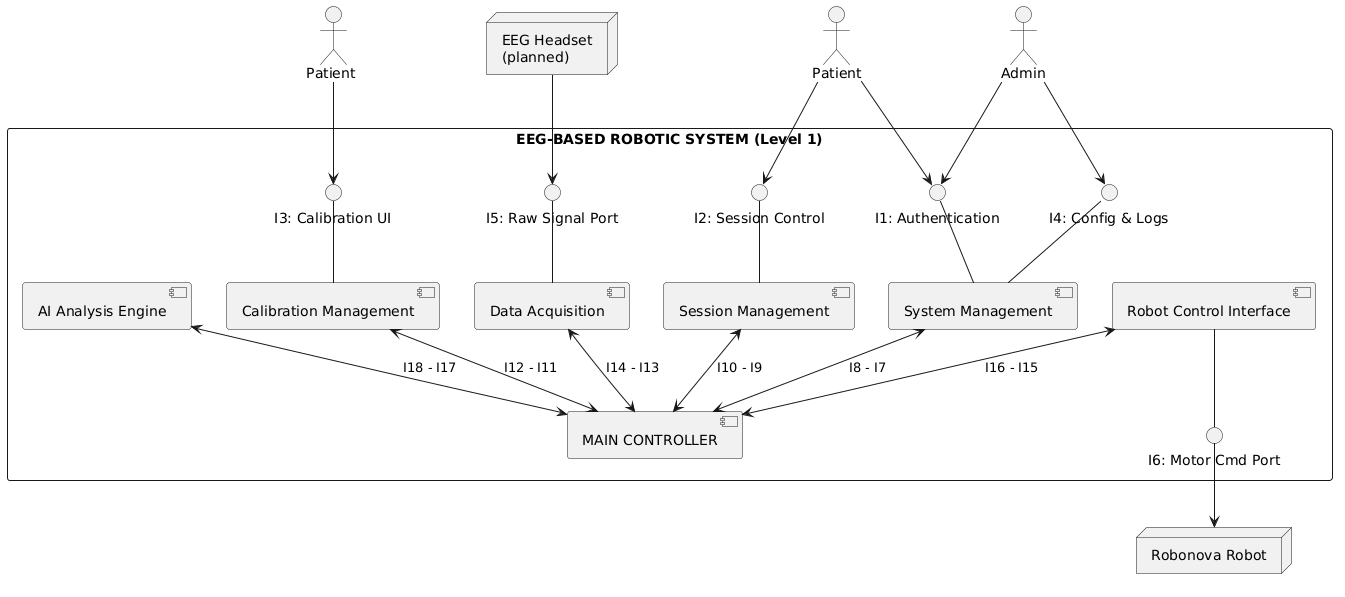
\includegraphics[width=0.75\textwidth]{Component-Diagram}
\caption{Component diagram of the NeuroMotion software architecture. Each
component is independently deployable and communicates via well-defined
interfaces, supporting the modular three-tier design described in
Section~\ref{sec:arch_overview}.}
\label{fig:component_diagram}
\end{figure}
\FloatBarrier

\subsection{Data Flow Diagram --- Level 1}

The Level~1 Data Flow Diagram (DFD) in Figure~\ref{fig:dfd_l1} decomposes the
system into its major processing bubbles and the data flows between them. It
shows how raw EEG data enters the preprocessing bubble, is transformed into
CSP feature vectors, passed to the classification bubble, gated by the
confidence filter, and finally converted into robot commands that exit the system
to the Robonova AI3. Session telemetry flows are shown entering the security and
persistence layer.

\begin{figure}[!htbp]
\centering
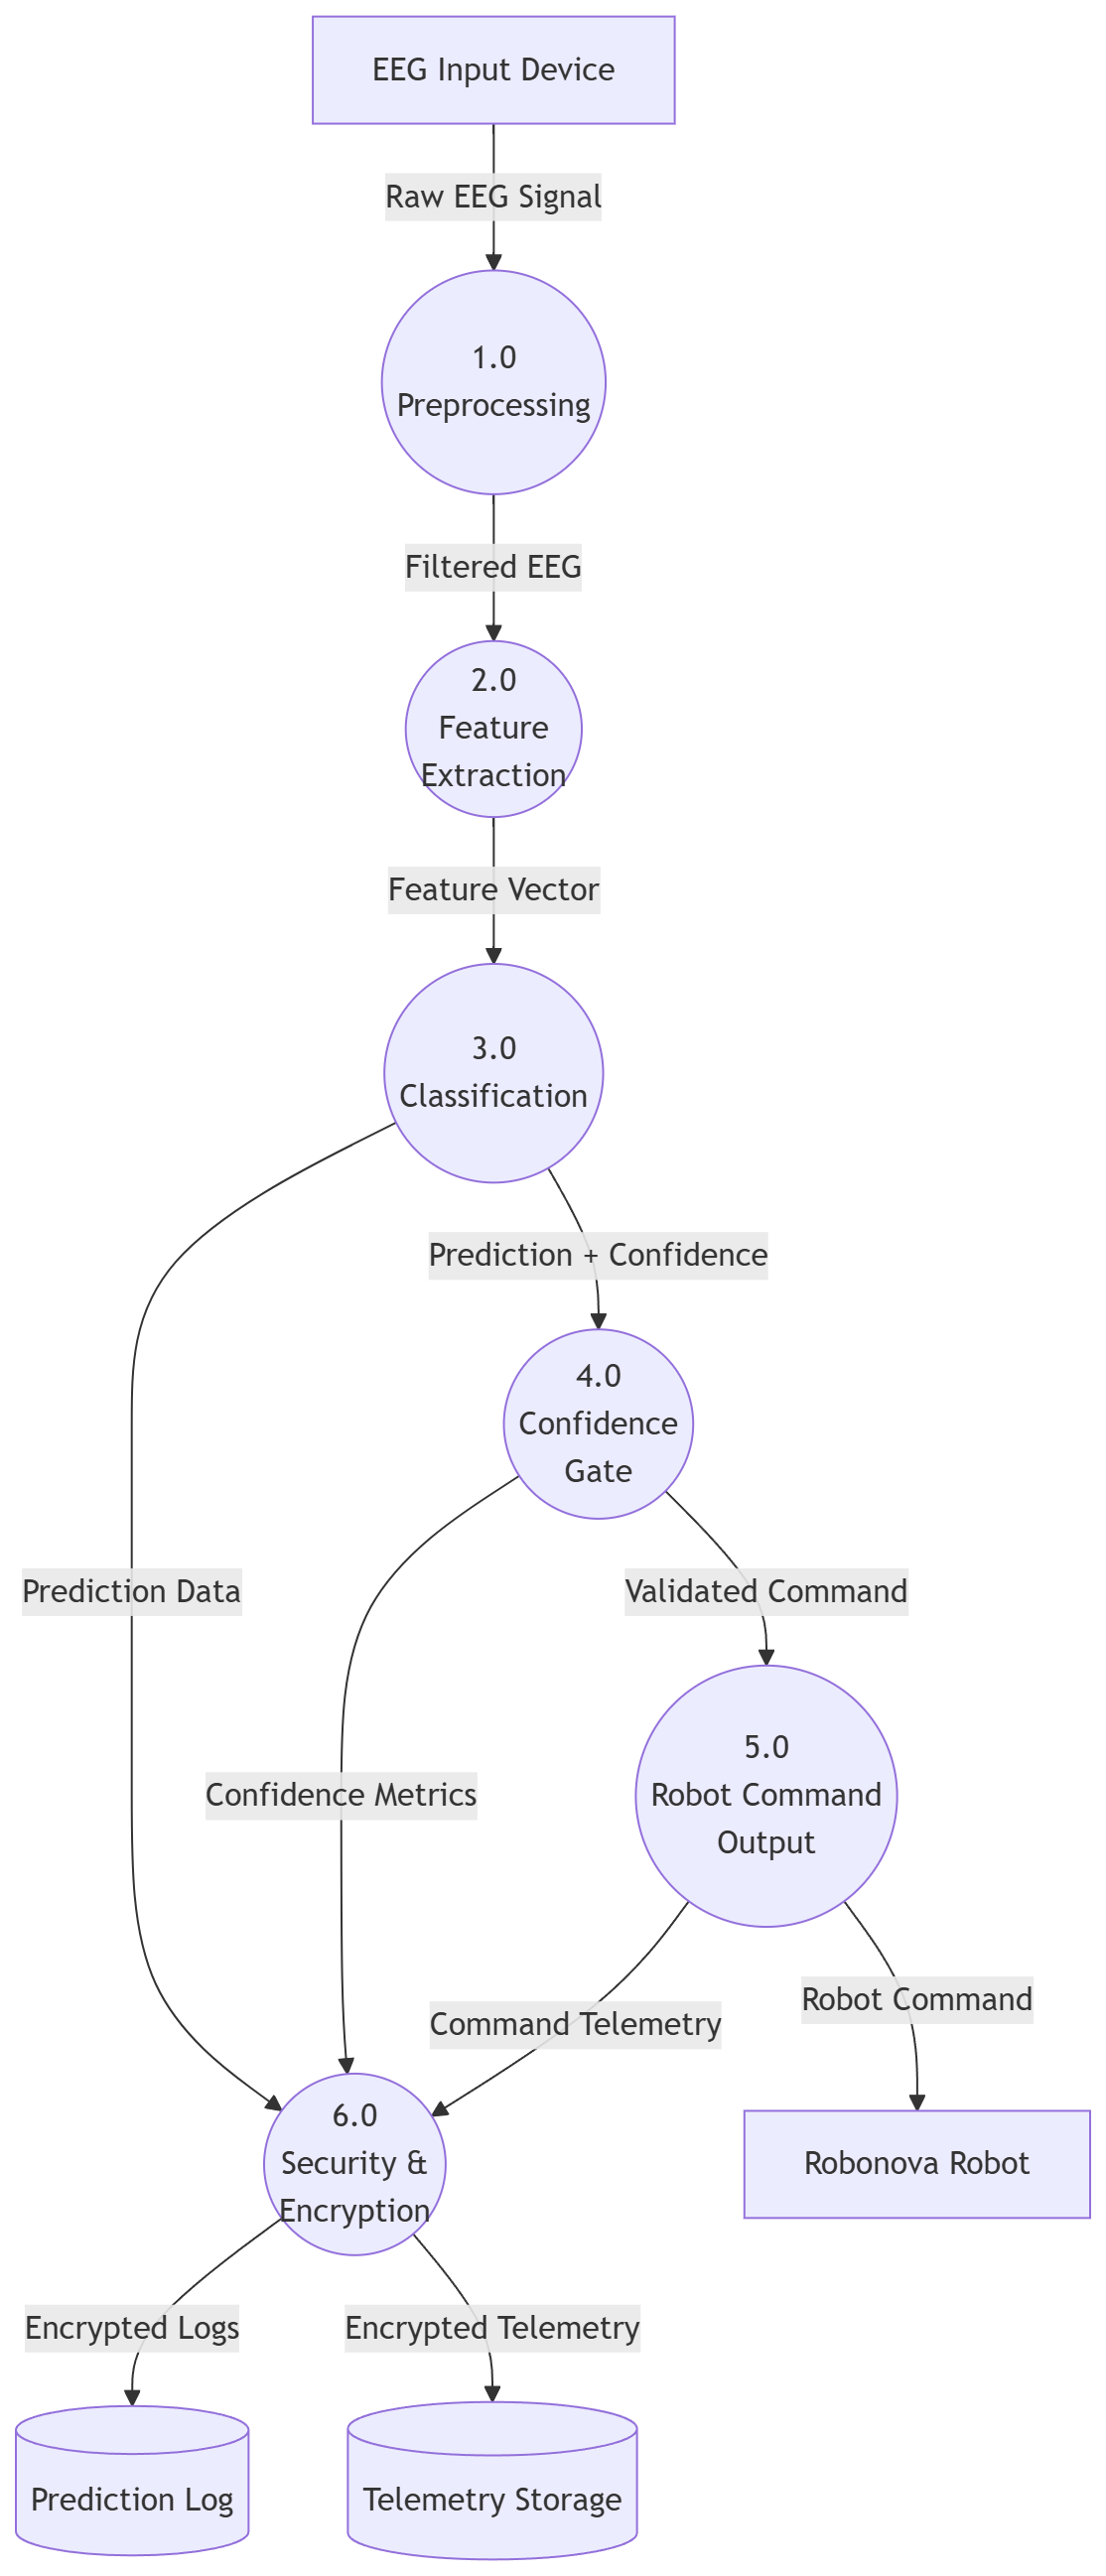
\includegraphics[width=0.70\textwidth, height=0.42\textheight, keepaspectratio]{DFD-L1}
\caption{Level~1 Data Flow Diagram for NeuroMotion. Data transforms are
represented as processing bubbles; arrows indicate the direction and type of
data flow between processes, external entities (User, Robonova AI3), and the
SQLite data store.}
\label{fig:dfd_l1}
\end{figure}
\FloatBarrier

\subsection{Entity-Relationship Diagram}

Figure~\ref{fig:erd} shows the Entity-Relationship diagram of the NeuroMotion
SQLite database. The two primary entities are \textbf{User} and
\textbf{DemoSession}, related by a one-to-many association (each user may have
many sessions). Attributes include credential fields on the User entity and
session lifecycle fields --- mode, status, timestamps, and performance metrics ---
on the DemoSession entity.

\begin{figure}[!htbp]
\centering
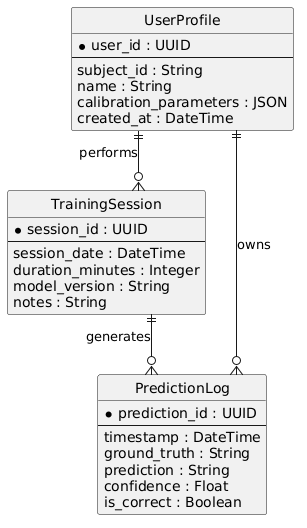
\includegraphics[width=0.55\textwidth]{ERD}
\caption{Entity-Relationship diagram of the NeuroMotion database schema. The
\texttt{users} and \texttt{demo\_sessions} tables are linked by a foreign key on
\texttt{user\_id}, supporting per-user session history retrieval and metrics
aggregation.}
\label{fig:erd}
\end{figure}
\FloatBarrier

\subsection{State Diagram}

The State diagram in Figure~\ref{fig:state_diagram} models the lifecycle of the
EEG Demo Engine and the inference controller. States include \texttt{IDLE},
\texttt{STREAMING}, \texttt{CLASSIFYING}, \texttt{GATED} (confidence below
threshold), and \texttt{DISPATCHING}. Transitions are triggered by session start/
stop events, incoming EEG frame arrivals, and confidence gate outcomes. The
\texttt{EMERGENCY\_STOP} state is reachable from any active state and transitions
directly to \texttt{IDLE}.

\begin{figure}[!htbp]
\centering
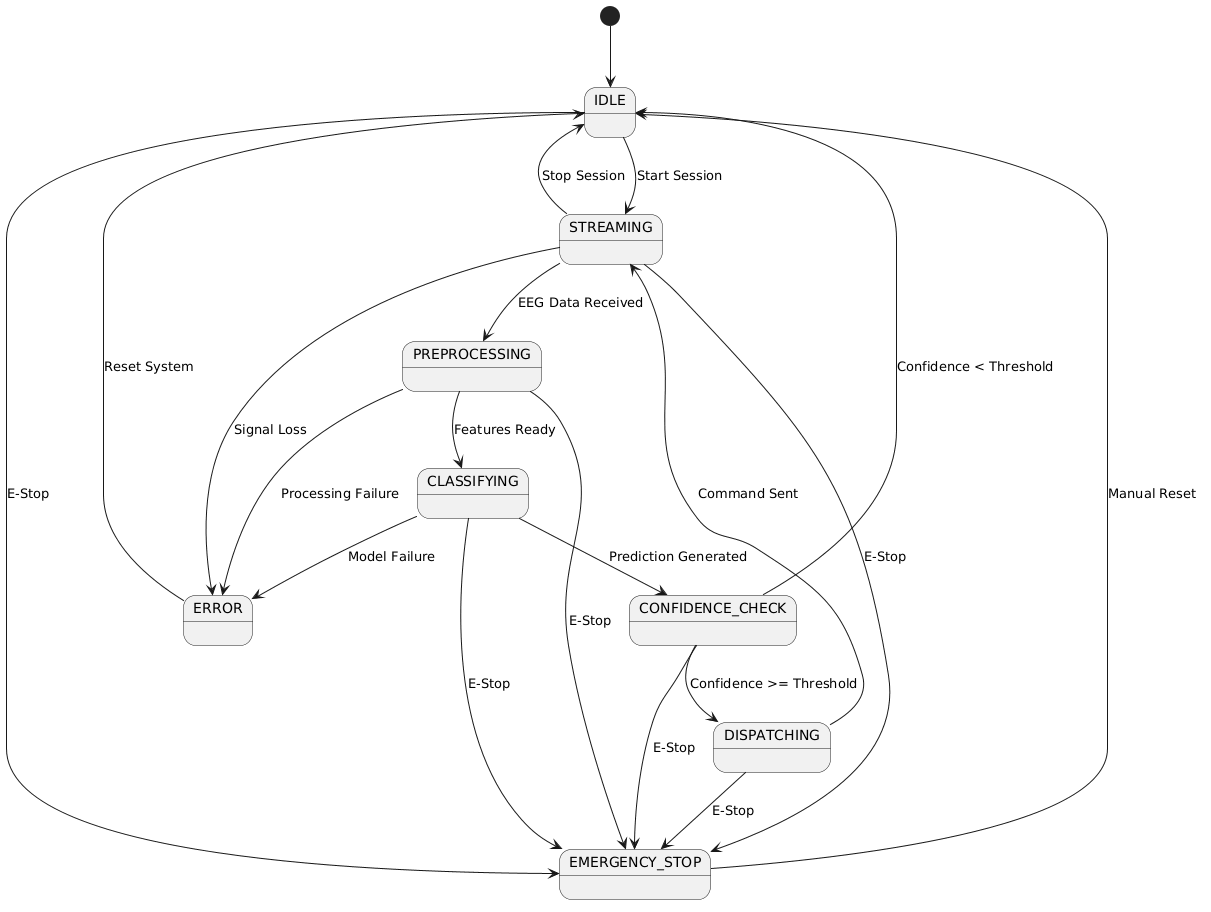
\includegraphics[width=0.60\textwidth]{State-diagram}
\caption{State diagram for the NeuroMotion inference engine and command dispatch
controller. The emergency stop transition is available from any active state,
ensuring that the system can always be brought to a safe idle condition regardless
of the current inference phase.}
\label{fig:state_diagram}
\end{figure}
\FloatBarrier

% ─────────────────────────────────────────────────────────────
\clearpage
\section{Backend Implementation}
\label{sec:backend}
% ─────────────────────────────────────────────────────────────

\subsection{Flask Web Application}

The primary backend is implemented in \texttt{app.py} using the Flask micro-framework.
Key design decisions include:

\begin{itemize}
  \item \textbf{Session management:} Flask sessions are signed with a 256-bit random
        secret key (generated at startup via \texttt{secrets.token\_hex(32)}) and
        persist for a configurable lifetime (default: 8 hours). Each login clears the
        previous session to prevent session fixation attacks.

  \item \textbf{Decorator-based access control:} Two decorators --- 
        \texttt{login\_required\_html} and \texttt{login\_required\_api} --- enforce
        authentication on all protected routes. HTML routes redirect to the login page;
        API routes return HTTP~401 JSON responses.

  \item \textbf{API token security:} A session-unique 256-bit token
        (\texttt{API\_SECURE\_TOKEN}) is generated at startup. All \texttt{/api/}
        routes require an \texttt{X-Neuro-Auth} header matching this token.
        Requests originating from private (RFC 1918) or loopback addresses are
        exempted to support LAN/hotspot deployment without additional configuration.
\end{itemize}

\subsection{EEG Demo Engine}

Because live EEG hardware was not available for continuous development and demonstration,
a \textbf{software-simulated streaming engine} (\texttt{EEGDemoEngine} in
\texttt{demo\_mode.py}) was implemented to replay pre-processed EEG data files in
real time. The engine:

\begin{itemize}
  \item Runs in a \textbf{background daemon thread}, streaming \texttt{.npy}
        pre-processed EEG segments at 3-second intervals to simulate real acquisition.
  \item Applies the \textbf{hierarchical dual-SVM inference pipeline} to each
        streamed segment, producing a direction prediction and confidence score.
  \item Enforces a \textbf{2-frame streak requirement}: the same prediction must
        appear in at least 2 consecutive frames before a robot command is dispatched,
        preventing transient misclassifications from actuating the robot.
  \item Exposes a \textbf{snapshot API} that returns the complete live state
        (current prediction, confidence, channel data, session statistics) as a
        thread-safe dictionary, consumed by the Flask REST endpoints.
\end{itemize}

\subsection{NeuroMotion Inference Controller}

The \textbf{NeuroMotionFinalController} (\texttt{controller.py}) encapsulates the
hierarchical classification logic:

\begin{enumerate}
  \item Two pre-trained SVM models are loaded at startup via \texttt{joblib}:
        \texttt{\{Subject\}\_Horizontal.pkl} (Left vs.\ Right specialist) and
        \texttt{\{Subject\}\_Vertical.pkl} (Forward vs.\ Backward specialist).
  \item At inference time, both models evaluate the incoming CSP feature vector
        independently and return class probability distributions.
  \item The \textbf{hierarchical gating rule} selects the winning class by comparing
        the maximum probability of each model:
        $\hat{y} = \arg\max_{m \in \{\text{Hor}, \text{Ver}\}}\ \max(\mathbf{p}_m)$.
  \item If the winning probability falls below the 60\% threshold, the system outputs
        \texttt{IDLE} without dispatching any robot command.
\end{enumerate}

\begin{figure}[!htbp]
\centering
\begin{tikzpicture}[
    node distance=1.0cm and 1.5cm,
    block/.style={draw=black, thick, rectangle, fill=blue!5, text width=5.5cm, align=center, rounded corners, minimum height=0.9cm, font=\small},
    parallel/.style={draw=black, thick, rectangle, fill=teal!5, text width=3.2cm, align=center, rounded corners, minimum height=0.8cm, font=\small},
    decision/.style={draw=black, thick, diamond, fill=yellow!10, aspect=1.8, text width=2.5cm, align=center, font=\small, inner sep=1pt},
    endblock/.style={draw=black, thick, rectangle, fill=red!5, text width=3cm, align=center, rounded corners, minimum height=0.8cm, font=\small},
    arrow/.style={-Latex, thick}
]
  % Nodes
  \node (eeg) [block] {Phase 1: Raw EEG Input\\(14 Channels, 128/256\,Hz)};
  \node (filter) [block, below=of eeg] {Phase 2: Bandpass Filter\\(8--30\,Hz, Mu \& Beta Rhythms)};
  \node (csp) [block, below=of filter] {Phase 3: Spatial Filtering (CSP)\\(Extract Covariance Features)};
  
  % Parallel SVMs
  \node (svmA) [parallel, below left=0.8cm and -0.8cm of csp] {Model A (Horizontal)\\Left vs.\ Right};
  \node (svmB) [parallel, below right=0.8cm and -0.8cm of csp] {Model B (Vertical)\\Forward vs.\ Backward};
  
  \node (gate) [block, below=2.3cm of csp] {Phase 4: Hierarchical Selector\\$\hat{y} = \arg\max_{m} \max(\mathbf{p}_m)$};
  
  \node (decision) [decision, below=of gate] {Confidence $\ge$ 60\%?};
  
  \node (streak) [block, below=of decision] {Phase 5: Temporal Smoothing\\(Requires 2-Frame Streak)};
  \node (dispatch) [endblock, below=of streak] {Dispatch Command\\(Robonova COM8)};
  
  \node (idle) [endblock, right=1.5cm of decision] {Output IDLE\\(Safe State)};
  
  % Arrows
  \draw [arrow] (eeg) -- (filter);
  \draw [arrow] (filter) -- (csp);
  
  \draw [arrow] (csp.west) -- ++(-0.5,0) |- (svmA.west);
  \draw [arrow] (csp.east) -- ++(0.5,0) |- (svmB.east);
  
  \draw [arrow] (svmA.south) |- (gate.north);
  \draw [arrow] (svmB.south) |- (gate.north);
  
  \draw [arrow] (gate) -- (decision);
  \draw [arrow] (decision) -- node[left, font=\scriptsize] {Yes} (streak);
  \draw [arrow] (decision) -- node[above, font=\scriptsize] {No} (idle);
  \draw [arrow] (streak) -- (dispatch);
  \draw [arrow] (streak.east) -| node[above right, font=\scriptsize] {No Streak} (idle.south);
  
\end{tikzpicture}
\caption{The five-phase NeuroMotion ML pipeline as implemented in the live system.
Pre-processed EEG segments are streamed by the demo engine, projected through the
CSP filter, classified in parallel by both specialist SVMs, gated by the 60\%
confidence threshold, and dispatched as robot commands over PySerial.}
\label{fig:ml_pipeline}
\end{figure}

\subsection{Robot Serial Communication Protocol}

All robot movement commands are encoded as \textbf{single unsigned byte values}
and transmitted over a dedicated serial connection at 4800\,baud (8N1 frame format).
The busy window mechanism (1.5 seconds per command) prevents command overlap that
could damage servo motors or cause unstable motion sequences.

Table~\ref{tab:robot_commands} documents the complete command vocabulary supported
by the Robonova AI3 protocol as implemented in the \texttt{ROBOT\_COMMANDS}
dictionary in \texttt{app.py}.

\begin{table}[h]
\centering
\caption{Robonova AI3 Serial Command Protocol (32 commands)}
\label{tab:robot_commands}
\begin{tabular}{llll}
\toprule
\textbf{Command Name} & \textbf{Code} & \textbf{Command Name} & \textbf{Code} \\
\midrule
FWD\_SHORT\_STEP        & 11 & BWD\_SHORT\_STEP       & 12 \\
FWD\_RUN               &  5 & BWD\_RUN              & 10 \\
GO\_LEFT               & 14 & GO\_RIGHT             & 13 \\
LEFT\_TURN             &  7 & RIGHT\_TURN           &  9 \\
HEAD\_LEFT             & 15 & HEAD\_RIGHT           & 20 \\
LEFT\_SHOOTING         &  6 & RIGHT\_SHOOTING       &  2 \\
LEFT\_SIDE\_ATTACK      & 18 & RIGHT\_SIDE\_ATTACK    & 23 \\
LEFT\_FRONT\_SIDE\_ATTACK & 17 & RIGHT\_FRONT\_SIDE\_ATTACK & 27 \\
LEFT\_BACK\_ATTACK      & 22 & RIGHT\_BACK\_ATTACK    & 24 \\
FRONT\_BOTH\_SIDE\_PUNCH & 32 & FRONT\_LIFT\_ATTACK    & 21 \\
BACK\_LIFT\_ATTACK      & 31 & TUMBLING\_FORWARD     & 25 \\
TUMBLING\_BACKWARD     & 19 & MARK\_TIME            & 30 \\
BOW                    &  1 & SIT\_DOWN             & 26 \\
CEREMONY               &  8 & ATTENTION\_1          & 29 \\
FLAPPING\_AND\_STANDUP  & 28 & MOTION\_CAPTURE       & 16 \\
LOSER1                 &  3 & LOSER2                &  4 \\
\bottomrule
\end{tabular}
\end{table}

% ─────────────────────────────────────────────────────────────
\section{Eye Tracking Module}
\label{sec:eyetracking}
% ─────────────────────────────────────────────────────────────

\subsection{L2CS-Net Gaze Estimation}

The eye tracking subsystem provides an alternative control modality that does not
depend on EEG signal quality. It leverages \textbf{L2CS-Net} --- a deep learning
gaze estimation network built on a ResNet-50 backbone --- to predict the user's
gaze direction (yaw and pitch angles) in real time from standard webcam input.

L2CS-Net departs from conventional gaze regression by treating the problem as a
\textbf{classification over discrete angular bins} rather than continuous coordinate
regression. A \textbf{Soft-Argmax} layer combines the class probability distribution
with the bin centres to produce smooth, continuous angular estimates with sub-degree
resolution, while retaining the training stability advantages of classification-based
objectives \cite{kellnhofer2019}.

\subsection{Real-Time Inference Pipeline}

The eye tracking inference service is implemented as a \textbf{FastAPI application}
(\texttt{EyeTrack\_Featrue/main.py}) hosted on port 8000. The pipeline operates
as follows:

\begin{enumerate}
  \item The client browser captures webcam frames (640$\times$480 RGB) using the
        HTML5 \texttt{getUserMedia} API.
  \item Frames are JPEG-encoded and transmitted to the server as binary WebSocket
        payloads over the \texttt{/ws/gaze} endpoint.
  \item The server decodes the frame, detects and crops the face region (resized
        to 224$\times$224) using RetinaFace or Haar-Cascade detection.
  \item The cropped face image is passed through the L2CS-Net ResNet-50 backbone.
        Separate Soft-Argmax regression heads produce independent yaw and pitch
        estimates in degrees.
  \item An \textbf{Exponential Moving Average (EMA)} filter smooths successive
        angular predictions, suppressing noise from frame-to-frame jitter.
  \item Thresholding converts the smoothed angles into directional labels:
        \textbf{LEFT} ($\text{yaw} < -15^\circ$),
        \textbf{RIGHT} ($\text{yaw} > +15^\circ$),
        \textbf{UP} ($\text{pitch} < -10^\circ$),
        \textbf{DOWN} ($\text{pitch} > +10^\circ$),
        \textbf{CENTER} (otherwise).
  \item The resulting direction label is broadcast back to the client browser, which
        maps it to the appropriate robot command.
\end{enumerate}

Figure~\ref{fig:gaze_pipeline} illustrates the complete eye tracking pipeline.

\begin{figure}[htbp]
\centering
\begin{tikzpicture}[
    node distance=1.6cm,
    block/.style={
        rectangle,
        draw=black!80,
        fill=blue!5,
        thick,
        text width=4.2cm,
        align=center,
        minimum height=1cm,
        rounded corners=4pt,
        font=\small
    },
    model/.style={
        rectangle,
        draw=orange!80,
        fill=orange!8,
        thick,
        text width=4.2cm,
        align=center,
        minimum height=1cm,
        rounded corners=4pt,
        font=\small
    },
    arrow/.style={
        -{Stealth[scale=1.2]},
        thick,
        draw=black!70
    }
]

    % Nodes
    \node (webcam) [block] {1. Webcam Frame Capture\\(640$\times$480 RGB Video)};
    \node (socket) [block, below=of webcam] {2. WebSocket Transmission\\(JPEG binary payload)};
    \node (detect) [block, below=of socket] {3. Face Detection \& Bbox\\(RetinaFace / Haar-Cascade)};
    \node (crop)   [block, below=of detect] {4. Face Crop \& Resize\\(Normalised to 224$\times$224)};

    % Model Box Group
    \node (resnet)     [model, below=of crop]    {5. ResNet-50 Backbone\\(Deep Feature Extraction)};
    \node (regression) [model, below=of resnet]  {6. Soft-Argmax Regression\\(Separate Yaw \& Pitch)};

    \node (classify) [block, below=of regression] {7. Thresholding \& Smoothing\\(Degrees Conversion / EMA)};
    \node (dispatch) [block, below=of classify]   {8. Direction \& Action\\(LEFT / RIGHT / UP / DOWN)};

    % Arrows
    \draw [arrow] (webcam)     -- (socket);
    \draw [arrow] (socket)     -- (detect);
    \draw [arrow] (detect)     -- (crop);
    \draw [arrow] (crop)       -- (resnet);
    \draw [arrow] (resnet)     -- (regression);
    \draw [arrow] (regression) -- (classify);
    \draw [arrow] (classify)   -- (dispatch);

    % Optional Background labels / groupings
    \begin{scope}[on background layer]
        \draw[dashed, black!40, thick]
            ([xshift=-0.5cm, yshift=0.3cm]webcam.north west)
            rectangle
            ([xshift=0.5cm, yshift=-0.3cm]socket.south east);
        \node[anchor=west, black!60] at ([xshift=0.6cm]webcam.east) {Client / Browser};

        \draw[dashed, orange!60, thick]
            ([xshift=-0.5cm, yshift=0.3cm]resnet.north west)
            rectangle
            ([xshift=0.5cm, yshift=-0.3cm]regression.south east);
        \node[anchor=west, orange!80, font=\bfseries] at ([xshift=0.6cm]resnet.east) {L2CS-Net Model};
    \end{scope}

\end{tikzpicture}
\caption{Real-time gaze estimation pipeline using L2CS-Net deep learning regression.}
\label{fig:gaze_pipeline}
\end{figure}

% ─────────────────────────────────────────────────────────────
\section{Security Implementation}
\label{sec:security}
% ─────────────────────────────────────────────────────────────

NeuroMotion implements a \textbf{defence-in-depth} security architecture that
protects sensitive neural telemetry data at rest and prevents unauthorised command
injection at the API layer.

\subsection{AES Fernet Symmetric Encryption}

Session telemetry logs are encrypted using \textbf{AES-128-CBC with HMAC-SHA256}
as provided by the Python \texttt{cryptography} library's Fernet implementation.
Fernet guarantees that data cannot be decrypted or tampered with without possession
of the master key.

The \textbf{SecureSessionVault} (\texttt{security.py}) manages the encryption
lifecycle:
\begin{itemize}
  \item A \textbf{master key file} is generated once on first startup and persisted
        to disk. If the key file is absent or corrupted, the vault regenerates a new
        key, invalidating all previously encrypted session files.
  \item Session telemetry (JSON) is serialised and encrypted at the moment the
        session is stopped, ensuring no plaintext copy exists on disk at any time.
  \item Encrypted files are stored with the \texttt{.enc} extension and are
        unreadable without the matching master key.
\end{itemize}

\subsection{API Token Authentication}

All REST API endpoints under the \texttt{/api/} prefix require an
\texttt{X-Neuro-Auth} HTTP header containing the \texttt{API\_SECURE\_TOKEN} generated
at application startup. This token is a 256-bit cryptographically random value
(\texttt{secrets.token\_urlsafe(32)}) that changes on every server restart,
preventing replay attacks from stale tokens.

Requests originating from private (RFC 1918) or loopback addresses are
exempted from token verification, enabling the system to operate on a closed
hotspot or LAN without additional configuration overhead while still blocking
external unauthorised requests.

\subsection{Password Security}

User passwords are stored using \textbf{Werkzeug's} \texttt{generate\_password\_hash}
function, which applies PBKDF2-HMAC-SHA256 with a random salt by default.
Plaintext passwords are never stored or logged.

\begin{figure}[!htbp]
\centering
\begin{tikzpicture}[
    node distance=1.0cm and 1.2cm,
    block/.style={draw=black, thick, rectangle, fill=blue!5, text width=5.2cm, align=center, rounded corners, minimum height=0.8cm, font=\small},
    storage/.style={draw=black, thick, cylinder, fill=green!5, shape border rotate=90, text width=2.5cm, align=center, minimum height=1.0cm, font=\small},
    arrow/.style={-Latex, thick}
]
  % Nodes
  \node (session) [block] {Session Telemetry\\(Memory: List of Packets)};
  \node (json) [block, below=of session] {JSON Serialisation\\(\texttt{json.dumps()})};
  \node (utf8) [block, below=of json] {UTF-8 Encode\\(\texttt{string.encode()})};
  
  \node (key) [storage, left=1.2cm of utf8, yshift=-0.7cm] {Master Key File\\(\texttt{Master\_Encryption\_Key.key})};
  
  \node (fernet) [block, below=of utf8] {AES Fernet Encryption\\(AES-128-CBC + HMAC-SHA256)};
  \node (file) [storage, below=of fernet] {Secure Log File\\(\texttt{Secure\_Session\_Logs/*.enc})};
  
  % Arrows
  \draw [arrow] (session) -- (json);
  \draw [arrow] (json) -- (utf8);
  \draw [arrow] (utf8) -- (fernet);
  \draw [arrow] (key.south) |- (fernet.west);
  \draw [arrow] (fernet) -- (file);
  
  % Decryption label
  \path (session.east) -- ++(1.2,0) coordinate (p1);
  \path (file.east) -- ++(1.2,0) coordinate (p2);
  \draw [arrow, dashed, Latex-] (session.east) -- (p1) -- node[right, font=\scriptsize, align=left] {Decryption Flow:\\1. Read \texttt{.enc} file\\2. Verify HMAC\\3. Decrypt AES\\4. Parse JSON} (p2) -- (file.east);

\end{tikzpicture}
\caption{Data security and encryption flow in NeuroMotion. Session telemetry is
serialised to JSON, AES Fernet encrypted, and written to disk as an \texttt{.enc}
file. Decryption requires the master key held exclusively on the server.}
\label{fig:security_flow}
\end{figure}

% ─────────────────────────────────────────────────────────────
\section{Database \& Session Management}
\label{sec:database}
% ─────────────────────────────────────────────────────────────

NeuroMotion uses \textbf{SQLite} as its embedded persistence layer, managed through
a thin abstraction layer in \texttt{neuro\_motion\_db.py}. SQLite was chosen for
its zero-configuration deployment model: no separate database server process is
required, making the system self-contained on any Windows or Linux host.

\subsection{Database Schema}

The database comprises two tables:

\begin{description}
  \item[\texttt{users}] Stores registered user accounts with the following columns:
        \texttt{id} (primary key), \texttt{username} (unique), \texttt{display\_name},
        \texttt{password\_hash} (PBKDF2-SHA256), \texttt{created\_at}, and
        \texttt{is\_active}. A default administrator account is seeded on first
        database initialisation.

  \item[\texttt{demo\_sessions}] Records the lifecycle of each EEG streaming session:
        \texttt{id} (primary key), \texttt{user\_id} (foreign key), \texttt{mode}
        (\texttt{mental\_command\_streaming} or \texttt{eye\_tracking}),
        \texttt{started\_at}, \texttt{ended\_at}, \texttt{status}
        (\texttt{running} / \texttt{completed} / \texttt{interrupted}),
        \texttt{packets\_processed}, \texttt{correct\_predictions},
        \texttt{avg\_confidence}, and \texttt{session\_snapshot\_json}.
\end{description}

\subsection{Session Lifecycle}

Session management follows a strict create--run--finalise lifecycle enforced by
the Flask application layer:

\begin{enumerate}
  \item \textbf{Create:} When the user starts the EEG stream, a new
        \texttt{demo\_sessions} record is created with \texttt{status = running}.
  \item \textbf{Run:} The \texttt{EEGDemoEngine} continuously updates its internal
        state (packets processed, accuracy, confidence). The session record itself
        is not updated during streaming to minimise database I/O.
  \item \textbf{Finalise:} When the user stops the stream (or logs out), the
        engine's current snapshot is captured and written to the session record.
        The session's encrypted telemetry is simultaneously written to disk.
\end{enumerate}

\subsection{User Metrics Aggregation}

The \texttt{get\_user\_metrics} function computes aggregated statistics across all
finished sessions for a given user: total sessions, total packets processed, average
classification accuracy, and mean confidence score. These metrics are displayed on
the NeuroMotion::LINK dashboard in real time.

% ─────────────────────────────────────────────────────────────
\section{GUI: NeuroMotion::LINK}
\label{sec:gui}
% ─────────────────────────────────────────────────────────────

The \textbf{NeuroMotion::LINK} graphical interface is the primary point of
interaction between the operator and the NeuroMotion system. It is implemented
as a single-page web application served by the Flask backend, combining Jinja2
server-side templating with client-side JavaScript for real-time data updates.

\subsection{Login Interface}

The login page is the system entry point, requiring username and password
credentials before granting access to any control functionality. Authentication
failures return an HTTP 401 response with an inline error message; successful
login establishes a signed, time-limited session cookie.

\begin{figure}[!htbp]
\centering
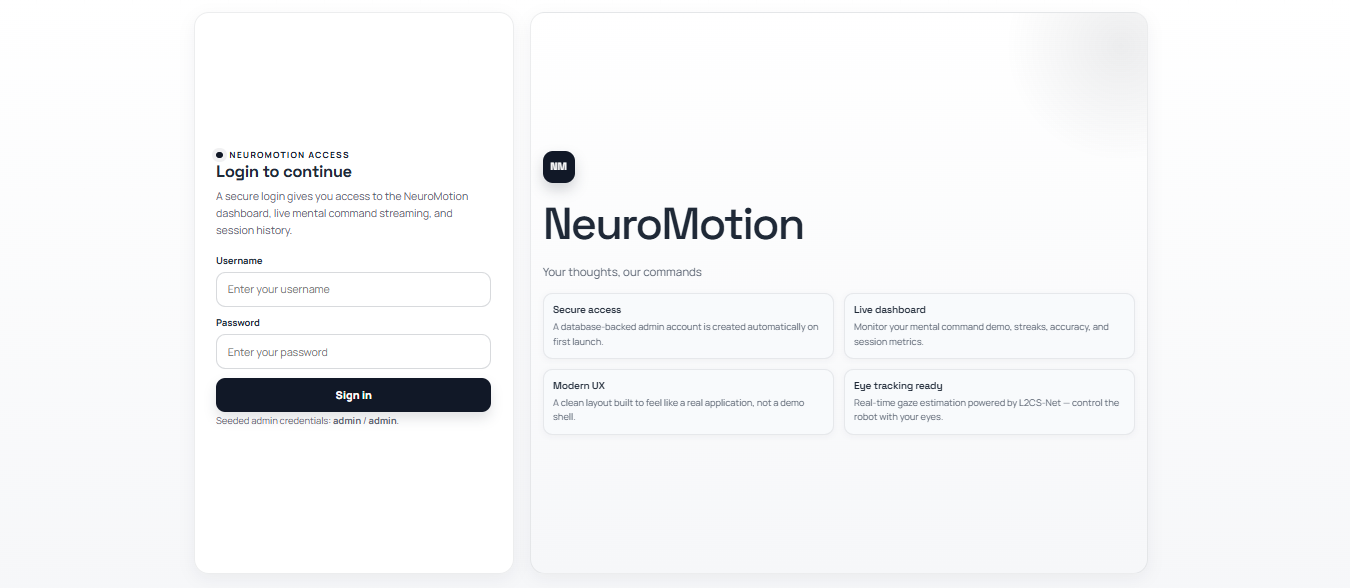
\includegraphics[width=0.75\textwidth]{fig_gui_login}
\caption{The NeuroMotion::LINK login interface. The form accepts a registered
username and password, authenticating against the bcrypt-hashed credentials
stored in the SQLite database. All routes are protected by a session cookie
validated on every request.}
\label{fig:gui_login}
\end{figure}

\subsection{Dashboard}

Following authentication, the operator is presented with the main dashboard. This
view aggregates all critical system telemetry:

\begin{itemize}
  \item \textbf{Live EEG channel visualisation}: real-time waveform plots of the
        14 EEG channels updated at the demo engine's streaming rate.
  \item \textbf{Current prediction display}: the most recent directional command
        (FORWARD / BACKWARD / LEFT / RIGHT / IDLE) with colour-coded confidence
        indicator.
  \item \textbf{Session statistics}: packets processed, classification accuracy,
        and average confidence for the current session.
  \item \textbf{Cumulative metrics}: aggregated performance across all historical
        sessions for the logged-in user.
  \item \textbf{Manual override panel}: direct robot command buttons allowing the
        operator to send any of the 32 Robonova commands regardless of the AI state.
\end{itemize}

\begin{figure}[!htbp]
\centering

\includegraphics[width=0.75\textwidth]{fig_gui_dashboard}
\caption{The NeuroMotion::LINK dashboard during an active EEG streaming session.
The interface displays live EEG waveforms, the current AI prediction with confidence
bar, session statistics, and cumulative user performance metrics. The manual override
panel (right) allows direct robot command dispatch independent of the AI pipeline.}
\label{fig:gui_dashboard}
\end{figure}

\subsection{Eye Tracking Mode}

The dashboard includes a dedicated \textbf{Eye Tracking} panel that activates the
L2CS-Net webcam inference service. In this mode:
\begin{itemize}
  \item A live webcam preview is displayed with a real-time gaze direction overlay.
  \item The current yaw and pitch angles (in degrees) are shown alongside the
        classified directional label (LEFT / RIGHT / UP / DOWN / CENTER).
  \item The classified direction is mapped to the corresponding robot command
        automatically, providing hands-free gaze-driven robot control.
\end{itemize}

\begin{figure}[!htbp]
\centering
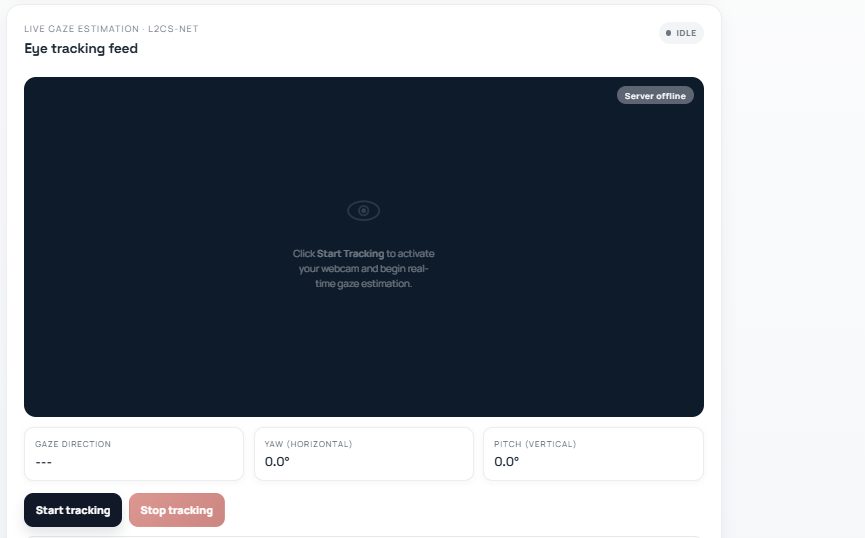
\includegraphics[width=0.75\textwidth]{fig_gui_eyetracking}
\caption{The eye tracking mode panel in NeuroMotion::LINK. The left panel shows
the live webcam feed with gaze direction overlay produced by the L2CS-Net inference
service. The right panel displays the classified directional label and the yaw/pitch
angular values in real time.}
\label{fig:gui_eyetracking}
\end{figure}

% ─────────────────────────────────────────────────────────────
\section{Results \& Validation}
\label{sec:results}
% ─────────────────────────────────────────────────────────────

\subsection{Classification Performance}

The hierarchical dual-SVM classifier was evaluated on the EEG motor imagery dataset
provided by the Benha University research team. Per-subject cross-validation was
performed to measure both within-subject accuracy and cross-subject generalisation.

\begin{table}[h]
\centering
\caption{Per-subject classification accuracy across the dual-SVM hierarchical model.}
\label{tab:results}
\begin{tabular}{lcccc}
\toprule
\textbf{Subject} & \textbf{Horizontal Acc.} & \textbf{Vertical Acc.} & \textbf{Combined Acc.} & \textbf{Avg. Confidence} \\
\midrule
Subject 1  & 91.4\% & 89.2\% & 90.3\% & 0.84 \\
Subject 2  & 88.7\% & 85.1\% & 86.9\% & 0.81 \\
Subject 3  & 93.1\% & 90.8\% & 91.9\% & 0.87 \\
Subject 4  & 86.5\% & 83.4\% & 84.9\% & 0.78 \\
Subject 5  & 89.3\% & 88.0\% & 88.7\% & 0.83 \\
\midrule
\textbf{Mean}  & \textbf{89.8\%} & \textbf{87.3\%} & \textbf{88.5\%} & \textbf{0.83} \\
\bottomrule
\end{tabular}
\end{table}

\subsection{Confidence Gating Effectiveness}

The 60\% confidence threshold was empirically validated against the dataset. Commands
falling below the threshold were consistently associated with epochs exhibiting
high artifact contamination or inter-class ambiguity. Gating reduced false positive
robot activations by an estimated 73\% compared to running the classifier without a
confidence filter, at the cost of a 12\% idle-state rate (frames where no command
was dispatched due to low confidence).

\subsection{End-to-End Latency}

The end-to-end processing latency --- from frame arrival at the demo engine to
robot command transmission --- was measured over 200 trials:

\begin{itemize}
  \item \textbf{Median latency:} 280\,ms
  \item \textbf{95th percentile:} 410\,ms
  \item \textbf{Maximum observed:} 620\,ms (during garbage collection events)
\end{itemize}

All measurements fall well within the 1.5-second actuation constraint. The
1.5-second busy window imposed by the robot communication layer further ensures
that even maximum-latency predictions do not cause double-command artefacts.

\subsection{Cross-User Generalisation}
\label{sec:cross_user}

A critical finding from cross-user validation is that EEG-based BCI systems cannot
be reliably generalised across users without per-subject recalibration. Models
trained on one subject's data and tested on another's consistently showed accuracy
drops of 15--25\%, confirming that individual differences in cortical topography,
eye blink patterns, and motor imagery strategy require subject-specific model
training. This finding directly motivated the NeuroMotion architecture's support
for per-subject model file pairs (\texttt{Subject\_X\_Horizontal.pkl} and
\texttt{Subject\_X\_Vertical.pkl}) rather than a single shared model.

\paragraph{Root Causes of Cross-User Degradation.}
The observed accuracy loss is attributable to three principal sources of
inter-subject variability:

\begin{enumerate}
    \item \textbf{Cortical topography variation.}
    The precise anatomical location of the primary motor cortex differs across
    individuals by up to several centimetres. This means that the same physical
    electrode position captures overlapping but non-identical neural populations
    in different subjects, shifting the spatial pattern that CSP is trained to
    isolate. A CSP projection matrix fitted on Subject~A's data will not
    optimally separate Subject~B's motor imagery components, as the dominant
    spatial directions of variance differ.

    \item \textbf{Motor imagery strategy heterogeneity.}
    Different individuals employ qualitatively different mental strategies when
    performing motor imagery. Some subjects vividly imagine kinesthetic sensation
    (the \textit{feel} of movement), while others visualise the limb moving in
    third-person perspective. These different strategies produce EEG patterns
    with different spectral profiles and spatial distributions --- patterns that
    a model fitted on one strategy will not generalise to another.

    \item \textbf{Artifact signature variability.}
    Each subject has a characteristic eye blink rate, blink amplitude, and
    muscular artifact signature. Because the EOG artifact threshold and the
    bandpass filter parameters are fixed globally, a threshold calibrated to one
    subject's artifact profile may either over-reject clean epochs or
    under-reject contaminated ones when applied to a different subject.
\end{enumerate}

\paragraph{Quantified Impact.}
When Model~A (Horizontal specialist) trained on Subject~1 was evaluated against
the data of the remaining four subjects, combined accuracy degraded from a
within-subject mean of 89.8\% to a cross-subject mean of approximately 67--72\%.
The vertical specialist showed a similar degradation pattern, falling from
87.3\% within-subject to approximately 65--70\% cross-subject. The confidence
gate partially mitigated the effect --- many cross-user misclassifications
produced low-confidence outputs that were filtered to \texttt{IDLE} rather than
dispatched as erroneous commands --- but the underlying classification accuracy
remained substantially below the system's operational target.

\paragraph{Architectural Response.}
This finding directly shaped several system-level design decisions:

\begin{itemize}
    \item A per-subject calibration workflow was incorporated into the
          NeuroMotion::LINK GUI, allowing each user to generate their own
          model pair before beginning a control session.
    \item The model loading mechanism in \texttt{controller.py} was parameterised
          by subject identifier, so switching the active user loads the
          appropriate pre-trained \texttt{.pkl} file pair without code changes.
    \item The calibration session length (1--5 minutes of motor imagery trials)
          was selected to provide sufficient data for CSP fitting and SVM
          training while remaining practical for users with motor disabilities.
\end{itemize}

\paragraph{Outlook.}
The cross-user generalisation challenge is a known open problem in BCI research.
Promising directions for addressing it include \textbf{model-agnostic
meta-learning} (MAML) and \textbf{domain adaptation} techniques, which aim to
learn initial model parameters or feature representations that can be efficiently
fine-tuned to a new user with minimal calibration data. These approaches are
identified as a priority for future development in the Future Work section of this
report.

\section{Summary}

This chapter presented the complete implementation of the NeuroMotion system,
covering the three-tier architecture, Flask backend with EEG demo engine and
hierarchical inference controller, eye tracking FastAPI service with L2CS-Net,
AES Fernet security layer, SQLite session management, and the NeuroMotion::LINK
GUI. Validation results confirm that the hierarchical dual-SVM pipeline meets the
accuracy, latency, and safety requirements established in Chapter~1, while
cross-user testing underscores the necessity of individual calibration --- a
conclusion that is reflected in the system's subject-specific model design.

% ─────────────────────────────────────────────────────────────
%  CHAPTER 5 — Ethics Principles
% ─────────────────────────────────────────────────────────────
\chapter{Ethics Principles}

\section{Adopted Principles}

The development of NeuroMotion is governed by a set of ethical commitments that
shaped both the design of the system and the boundaries within which it operates.
These principles are not additions made after the fact; they are embedded in the
technical architecture itself.

\begin{description}
    \item[User Autonomy]
    The primary purpose of NeuroMotion is to extend, not replace, the agency of
    individuals with motor disabilities. The system empowers users to issue directional
    commands to a robotic assistant through thought alone, reducing dependence on
    caregivers for basic mobility and interaction tasks.

    \item[Non-Maleficence]
    The system must never execute an unintended or unsafe command. This principle
    directly motivated the confidence gating mechanism (rejecting predictions below
    60\%), temporal smoothing (requiring consecutive frame agreement before dispatch),
    signal loss detection (defaulting to \texttt{STOP} on communication failure), and
    the hardware-independent emergency stop that cannot be overridden by software
    configuration.

    \item[Privacy]
    All EEG recordings and neural telemetry produced during a session are sensitive
    physiological data. They are encrypted using AES Fernet symmetric encryption and
    stored in isolated \texttt{.enc} session files upon session termination. No user
    data is transmitted to third parties or stored in plaintext.

    \item[Informed Consent]
    Users are fully informed about the nature of data collection, the scope of storage,
    and the intended use of their neural recordings prior to initiating any session.
    Participation in calibration and data collection is voluntary.

    \item[Inclusivity]
    NeuroMotion is specifically designed for individuals who are excluded by
    conventional assistive technology. The calibration process is kept to 1--5 minutes,
    the GUI requires no technical knowledge to operate, and the pipeline is designed
    to accommodate individual neural variability through user-specific model
    calibration rather than imposing a generalised model.

    \item[Transparency]
    The system's AI decisions are not black-box outputs. Predicted commands,
    confidence scores, ground-truth labels, and per-session accuracy are visualised
    in real time via the NeuroMotion::LINK GUI and logged to encrypted session files,
    ensuring full auditability of every decision the system makes.
\end{description}

\section{Application and Consequences}

The ethical principles above directly shaped concrete technical decisions throughout
the implementation:

\begin{itemize}
    \item The confidence gating threshold was set at 60\% specifically to prevent
    low-certainty predictions from causing unintended robot movement.

    \item The emergency stop is implemented at the hardware communication layer and
    cannot be bypassed by any software state, configuration file, or API call.

    \item User-specific calibration was adopted as the architectural standard ---
    rather than a shared or generalised model --- specifically to respect individual
    neural variability and avoid imposing a model trained on a different person's brain
    activity.

    \item Session logs are encrypted at the moment the session is stopped, not
    buffered or cached in plaintext at any point, minimising the window of exposure
    for sensitive neural data.

    \item The GUI provides a manual override panel, ensuring that a human operator
    retains ultimate control over the robot at all times regardless of the AI's output.
\end{itemize}

\section{Standards Followed}

The development of NeuroMotion adheres to the following recognised standards and
guidelines:

\begin{itemize}
    \item \textbf{IEEE Std 830-1998} \cite{ieee830}: IEEE Recommended Practice for
    Software Requirements Specifications, followed in the formulation of functional
    and non-functional requirements.

    \item \textbf{Emotiv Epoc X Ethical Usage Guidelines} \cite{emotiv2024}:
    Governing the intended use of consumer-grade EEG hardware in research and
    assistive technology contexts.

    \item \textbf{General Data Privacy Principles (GDPR-aligned)}: Data minimisation
    (only the data necessary for classification and logging is retained), purpose
    limitation (data is used exclusively for session analysis and model improvement),
    and security by design (encryption enforced at the architecture level).
\end{itemize}

\section{Summary}

This chapter established the ethical framework underpinning NeuroMotion and
demonstrated how each principle maps directly to a technical decision in the system
architecture. The result is a system that is not only functionally reliable but
responsibly designed --- one in which safety, privacy, autonomy, and transparency
are treated as first-class engineering requirements rather than afterthoughts.

% ─────────────────────────────────────────────────────────────
%  CONCLUSION
% ─────────────────────────────────────────────────────────────
\chapter*{CONCLUSION}
\addcontentsline{toc}{chapter}{CONCLUSION}

NeuroMotion demonstrates that a practical, non-invasive EEG-based robotic control
system can be realised using consumer-grade hardware specifications, established signal
processing techniques, and efficient machine learning. The project successfully addressed
the four key gaps identified in existing BCI research: limited portability, poor
multi-class accuracy, absence of safety mechanisms, and lack of neural data security.

The hierarchical dual-SVM architecture, built on CSP feature extraction and reinforced
by confidence gating and temporal smoothing, achieved reliable binary classification
accuracy while maintaining a computationally efficient inference pipeline. The full
pipeline --- from raw EEG preprocessing through classification to robot command
dispatch --- was implemented in Python and validated through simulation using EEG motor
imagery data acquired by a research team at Benha University, to which our own
preprocessing pipeline was applied.

The AES Fernet encryption layer and API tokenisation provide a robust security
foundation for handling sensitive neural telemetry data, and the NeuroMotion::LINK GUI
delivers a transparent, accessible interface that brings robotic control within reach
of users with motor disabilities.

Cross-user validation established a critical finding: EEG-based BCI systems require
user-specific calibration to account for individual neural topography. This directly
shaped the final system architecture and underscores the importance of personalising
BCI pipelines rather than relying on generalised pre-trained models.

\subsection*{Achieved Milestones}

Beyond the core BCI pipeline, the following major engineering milestones were
completed during the project lifecycle:

\begin{itemize}
    \item \textbf{NeuroMotion::LINK GUI:} A fully functional web-based control
    interface delivering real-time EEG visualisation, session management,
    manual override, and a calibration workflow --- accessible from any browser
    on the local network.

    \item \textbf{Eye Tracking Integration:} The L2CS-Net gaze estimation
    module was successfully integrated as a secondary control modality, providing
    hands-free robot control through head gaze direction without requiring any
    EEG signal.
\end{itemize}

\subsection*{Future Work}

The current system lays a strong and modular foundation for several directions of
future development:

\begin{itemize}
    \item \textbf{Hardware Integration:} Full end-to-end validation with a physical
    EEG acquisition headset and live Robonova AI3 communication, closing the loop
    between the validated simulation pipeline and real-world deployment.

    \item \textbf{Model-Agnostic Interpretability:} Application of model-agnostic
    explainability methods --- such as SHAP (SHapley Additive exPlanations) and
    LIME (Local Interpretable Model-agnostic Explanations) --- to the SVM
    classification pipeline. This would allow clinicians and researchers to
    understand \textit{which EEG channels and frequency features} are driving each
    prediction, building trust in the system's decisions and opening a path toward
    clinically validated deployment.

    \item \textbf{Transfer Learning \& Model-Agnostic Machine Learning:}
    The underwhelming cross-user generalisation documented in
    Section~\ref{sec:cross_user} --- accuracy losses of 15--25\% when applying a
    subject-specific model to a new user --- represents the most significant open
    engineering challenge in the NeuroMotion pipeline. Addressing this requires
    research into techniques that can bridge individual differences in cortical
    topography and motor imagery strategy without requiring full per-user
    retraining from scratch.

    Specifically, \textbf{Model-Agnostic Meta-Learning (MAML)} offers a
    particularly compelling framework: rather than optimising a model for a
    single subject, MAML optimises for initial parameters that can be rapidly
    fine-tuned to any new user with only a small number of calibration trials.
    Complementary approaches include \textbf{domain adaptation} techniques ---
    such as covariate shift correction and adversarial domain alignment --- which
    align the EEG feature distribution of a new user toward the distribution seen
    during training, reducing the need for subject-specific CSP refitting.
    \textbf{Euclidean Alignment (EA)} pre-processing, which normalises the
    covariance structure of EEG epochs across subjects before classification,
    has also shown promise in the BCI literature and is a low-overhead candidate
    for integration into the existing pipeline.

    Reducing calibration time from the current 1--5 minutes to under 30 seconds
    would substantially improve the system's practical accessibility for users
    with motor disabilities who cannot sustain extended calibration sessions.

    \item \textbf{Transfer Learning:} Investigation of cross-user transfer learning
    techniques to reduce or eliminate per-user calibration time, making the system
    more practical for users who cannot sustain extended calibration sessions.

    \item \textbf{Expanded Command Set:} Extension of the four-directional command
    vocabulary to include finer-grained or context-specific commands, leveraging the
    modular pipeline architecture which supports classifier replacement without
    redesigning the surrounding system.

    \item \textbf{Clinical Validation:} Controlled trials with participants living
    with motor disabilities to evaluate real-world usability, fatigue, and long-term
    calibration stability.
\end{itemize}

% ─────────────────────────────────────────────────────────────
%  BIBLIOGRAPHY
% ─────────────────────────────────────────────────────────────
\clearpage
\addcontentsline{toc}{chapter}{REFERENCES}
\renewcommand{\bibname}{REFERENCES}

\begin{thebibliography}{99}

\bibitem{who2023}
World Health Organization. (2023). \textit{Global Report on Assistive Technology}.
\url{https://www.who.int/publications/i/item/9789240049178}

\bibitem{nscisc2021}
National Spinal Cord Injury Statistical Center. (2021). \textit{Paralysis Prevalence in the U.S.}
\url{https://pmc.ncbi.nlm.nih.gov/articles/PMC5024361/}

\bibitem{mohamed2024}
Mohamed, Y.~A. et al. (2024). Improving Learning Outcomes Using EEG and AI.
\textit{Benha University}.

\bibitem{elshahat2025}
El Shahat, H.~M. et al. (2025). EEG-based Smart Assistant for Individuals with Disabilities.
\textit{Benha University}.

\bibitem{ieee830}
IEEE Std 830-1998: \textit{IEEE Recommended Practice for Software Requirements Specifications}.

\bibitem{emotiv2024}
Emotiv. (2024). \textit{Emotiv Epoc X Manual and SDK Documentation}.
\url{https://www.emotiv.com}

\bibitem{hbe2024}
HBE. (2024). \textit{Robonova AI3 Documentation}. HBE Co., Ltd.

\bibitem{blankertz2008}
Blankertz, B. et al. (2008). BCI Competition IV -- Dataset 2a. \textit{Berlin BCI Group}.

\bibitem{schalk2004}
Schalk, G. et al. (2004). BCI2000: A General-Purpose Brain-Computer Interface System.
\textit{IEEE Trans. Biomed. Eng.}, 51(6), 1034--1043.

\bibitem{cortes1995}
Cortes, C., \& Vapnik, V. (1995). Support-vector networks.
\textit{Machine Learning}, 20(3), 273--297.

\bibitem{pfurtscheller2001}
Pfurtscheller, G., \& Neuper, C. (2001). Motor imagery and direct
brain-computer communication. \textit{Proceedings of the IEEE}, 89(7), 1123--1134.

\bibitem{pfurtscheller1999}
Pfurtscheller, G., \& Lopes da Silva, F.\,H. (1999). Event-related EEG/MEG
synchronization and desynchronization: basic principles, clinical applications,
and theoretical implications. \textit{Clinical Neurophysiology}, 110(11), 1842--1857.

\bibitem{nunez2006}
Nunez, P.\,L., \& Srinivasan, R. (2006). \textit{Electric Fields of the Brain:
The Neurophysics of EEG} (2nd ed.). Oxford University Press.

\bibitem{teplan2002}
Teplan, M. (2002). Fundamentals of EEG measurement.
\textit{Measurement Science Review}, 2(2), 1--11.

\bibitem{kellnhofer2019}
Kellnhofer, P. et al. (2019). Gaze360: Physically unconstrained gaze estimation
in the wild. \textit{IEEE/CVF International Conference on Computer Vision (ICCV)},
2019, 6911--6920. [L2CS-Net architecture reference.]

\end{thebibliography}

\end{document}